\chapter{Konzeption}
\label{chap:Konzept}

%To DOs für dieses Kapitel: Tabellen überarbeiten, Texte überarbeiten/anpassen, Kapiteleinleitungen und fehlende Abschnitte schreiben, Quellen einfügen (vgl. Kommentare Overleaf), Bezug zu FF1 herstellen

In diesem Kapitel wird die Konzeption der beiden binären Interaktionsschnittstellen dargelegt. Diese Konzeption bildet das Fundament dieser Arbeit, da sie die Grundlage für die spätere Implementierung und Evaluation legt. Der Prozess folgt einem systematischen Ablauf, der auf den Grundprinzipien der morphologischen Analyse von \citet{10.1007/978-3-642-87617-2_14} basiert und für den spezifischen Kontext dieser Arbeit angepasst wurde. Diese Methode ermöglicht eine strukturierte und umfassende Betrachtung des Design Space. Der Ablauf besteht aus vier zentralen Schritten:

\begin{itemize}
    \item \textbf{Definition des Design Space:}
    In diesem Schritt werden die grundlegenden Gestaltungsmöglichkeiten und Anforderungen für die Interaktionen erarbeitet. Dazu werden die für die Zielsetzung dieser Arbeit relevanten Interaktionsaufgaben abgeleitet sowie Interaktionskomponenten und -Parameter identifiziert.
    \item \textbf{Erarbeitung konkreter Ausprägungen:}
    Auf Grundlage des definierten Design Space werden spezifische Ausprägungen für die Interaktionsaufgaben und -komponenten entwickelt, die die Bandbreite möglicher Ansätze abbilden.
    \item \textbf{Einordnung anhand der Parameter:}
    Die erarbeiteten Optionen werden systematisch anhand der zuvor identifizierten Parameter eingeordnet. Dieser Schritt dient dazu, die Designentscheidungen transparent darzulegen und zu begründen.
    \item \textbf{Ableitung der finalen Konzepte:}
    Abschließend werden die finalen Konzepte für die beiden binären Interaktionsschnittstellen abgeleitet, die anschließend im Prototyp implementiert werden.
\end{itemize}
 
Durch diese strukturierte Vorgehensweise wird die erste Forschungsfrage (FF1) adressiert.   

\section{Definition des Design Space}

Die Beschreibung des Design Space für binäre Interaktionen in PaneoVR basiert auf einer hierarchischen Struktur mit drei Ebenen. Die grundlegende Ebene wird durch die Interaktionsaufgaben definiert, die die für die Nutzung der Anwendung erforderlichen Interaktionsarten umfassen. Die zweite Ebene umfasst die Interaktionskomponenten, die spezifische Teilaspekte der Interaktion näher bestimmen. Die letzte Ebene bilden die Parameter. Parameter beschreiben in diesem Kontext Designüberlegungen, anhand derer die Interaktionstechniken und -ausprägungen bewertet werden. Die definierten Parameter beeinflussen dabei das gesamte VR-Erlebnis \citep{10.1145/3441852.3471230}. Die Kombination verschiedener Ausprägungen von Interaktionsaufgaben und -komponenten aus diesem Design Space kann anschließend als Grundlage für die Entwicklung neuartiger Interaktionstechniken verwendet werden.

{\normalfont \bfseries Interaktionsaufgaben:}  

Die Nutzung der mit PaneoVR erstellten Trainings basiert auf zwei grundlegenden Interaktionsaufgaben. Die erste Interaktionsaufgabe besteht in der Selektion von Interaktionselementen innerhalb der Szene, d.h. von Elementen wie z. B.  Wegpunkten oder Dialogfeldern, sowie von UI-Elementen, z. B. innerhalb des Hauptmenüs. Die zweite Interaktionsaufgabe umfasst die Navigation innerhalb der Szene. Dies umfasst die Änderung der Blickrichtung innerhalb der Szene. Da PaneoVR keinen dreidimensionalen Navigationsraum bereitstellt, sondern lediglich 360°-Videos präsentiert, ist eine klassische Navigation im 3D-Raum nicht notwendig. Stattdessen genügt eine Rotation der Szene, um die Blickrichtung zu ändern und damit innerhalb der virtuellen Welt zu navigieren. Da davon auszugehen ist, dass Nutzende mit motorischen Beeinträchtigungen Kopfbewegungen nicht frei und ohne Einschränkungen ausführen können, ist die Entwicklung einer alternativen Navigationsform unabdingbar. 

{\normalfont \bfseries Interaktionskomponenten:} 
%Überlegung: Ist Fehlerkorrektur eine Komponente? 

In Bezug auf die Interaktionen in PaneoVR lassen sich insgesamt drei verschiedene Komponenten identifizieren, deren konkrete Ausgestaltung einen direkten Einfluss auf die Erfahrung nimmt. 

Die Komponente Display definiert Darstellung und Integration des Interaktionsverfahren in die virtuelle Umgebung. Im Rahmen der Festlegung der Interaktionskomponente ist insbesondere zu bestimmen, ob sich die Interaktion auf das Sichtfeld des Nutzenden beschränkt. Die Relevanz dieser Komponente zeigt sich insbesondere in Kontexten, in denen Nutzende in der Lage sind, ihren Kopf zu bewegen und damit ihr Blickfeld unabhängig von der binären Interaktionsschnittstelle zu verschieben.

Eine weitere zu berücksichtigende Komponente ist die Transition. Diese ist insbesondere bei der Betrachtung des Navigationsprozesses von Bedeutung. Die Transition beschreibt die Art und Weise, wie die Drehung der First-Person-Kamera erfolgt, wenn Nutzende eine navigationsbezogene Interaktion durchführen. Das heißt, Transition beschreibt den Übergang zwischen der aktuellen und der neuen Blickrichtung.

Die letzte relevante Komponente ist die Initialisierung. Dabei wird festgelegt, ob das gewählte Interaktionsverfahren automatisch und kontinuierlich aktiv ist oder zunächst durch eine initiale Interaktion initialisiert werden muss. 

{\normalfont \bfseries Parameter:} 

Die Entwicklung und Bewertung von Interaktionen basiert in der Regel auf der Berücksichtigung verschiedener Parameter, welche das Gesamterlebnis einer VR-Anwendung maßgeblich beeinflussen \citep{10.1145/3441852.3471230}. Die relevanten Parameter für die Interaktionen in PaneoVR werden auf Basis vorangegangener Forschungsarbeiten identifiziert. Da die Gewährleistung einer guten Usability das primäre Ziel der Gestaltung von Interaktionen in VR darstellt \citep{dorner_virtual_2019}, werden die Parameter Effizienz \citep{DINISO9241-11}, Effektivität \citep{DINISO9241-11}, Erlernbarkeit \citep{DINISO9241-110} sowie Robustheit \citep{DINISO9241-110} definiert. Darüber hinaus werden die Parameter Interaktionsgeschwindigkeit \citep{COOK2015117} und Komfort \citep{jerald_vr_2016} berücksichtigt. 

\textit{Effizienz} beschreibt das Verhältnis zwischen den eingesetzten Ressourcen und dem damit erreichten Ziel \citep{DINISO9241-11}. Im Anwendungskontext ist  insbesondere der benötigte Aufwand als relevante Ressource zu betrachten.

\textit{Effektivität} bezeichnet die Genauigkeit und Vollständigkeit, mit der Benutzer ihre Ziele erreichen. Sie beschreibt, inwieweit die tatsächlichen Ergebnisse mit den angestrebten übereinstimmen. Je nach Kontext kann die Genauigkeit entweder anhand der Korrektheit eines Ergebnisses oder anhand des Erreichens eines akzeptablen Grads der Übereinstimmung mit dem Ziel bewertet werden \citep{DINISO9241-11}.

\textit{Erlernbarkeit} beschreibt das Ausmaß, in dem eine Interaktion ohne vorherige Einarbeitung verstanden und genutzt werden kann. In diesem Kontext ist von Relevanz, dass insbesondere ein hoher Wiedererkennungswert der Interaktion eine einfache und intuitive Bedienbarkeit bedingt \citep{jerald_vr_2016}.

\textit{Robustheit} beschreibt die Fähigkeit eines Systems, auf Fehler von Nutzenden angemessen zu reagieren \citep{DINISO9241-110}. Im Rahmen dieser Betrachtung wird untersucht, welche Maßnahmen ergriffen werden, um das Auftreten von Fehlern zu verhindern und inwiefern eine Korrektur von Fehlern möglich ist.

\textit{Interaktionsgeschwindigkeit} beschreibt die Zeit, die benötigt wird, um ein Interaktionsziel zu erreichen. Es wird somit die Zeit betrachtet, die für die Ausführung einer Interaktionsaufgabe benötigt wird. Im Rahmen dieser Betrachtung wird insbesondere die Wartezeit während der Interaktion analysiert.  

\textit{Komfort} bezeichnet die Wahrnehmung der Nutzenden bezüglich der Angenehmheit der Interaktion \citep{jerald_vr_2016}. In diesem Zusammenhang ist insbesondere die Wahrscheinlichkeit des Auftretens von Motion Sickness von Bedeutung. Dabei werden Faktoren wie Ermüdung, erhöhte Konzentration und visuelle Komplexität in die Bewertung einbezogen.

\section{Ausprägungen der Interaktionsaufgaben und Komponenten}

Folgend werden mögliche Ausprägungen zur Implementierung der zuvor beschriebenen Interaktionsaufgaben und Komponetnen erörtert.

{\normalfont \bfseries Interaktionsaufgaben}  

1. Selektion: 

Die Realisierung einer binären Interaktion erfordert die Implementierung einer indirekten Selektionsmethode. In diesem Zusammenhang sind Scanning-Verfahren eine der am weitesten verbreiteten Methoden \citep{COOK2015117}. Zur Implemntierung in PaneoVR werden die gängigen Scanning-Verfahren Automatic Item Scanning, Step Item Scanning mit Dwell Selection, Inverse Item Scanning sowie Continueous Cartesian Scanning (vgl. \autoref{subchap:Scanning}) in Betracht gezogen. 

2. Navigation:

Im Sinne einer konsistenten Gestaltung sollte die Art der Interaktion bei der Navigation einheitlich zu der bei der Selektion sein. Damit soll erreicht werden, dass sich das System für die Nutzenden möglichst erwartungskonform verhält. In dieser Konsequenz bedingt sich die Auswahl der Ausprägungen gegenseitig.

In der Literatur liegen bisher keine konkreten Umsetzungen für binäre Navigationsschnittstellen in VR vor. Ein Ansatz, den bspw. \citet{wentzel_bring-your-own_2023} beschreibt, wäre die Übertragung von bereits existierenden Accessibility-Techniken für Smartphones auf den Einsatz in VR. Eine weit verbreitete Technik bei Smartphones besteht darin, dass sich ein Cursor von links nach rechts über den Bildschirm bewegt und der Nutzende durch das Drücken eines Schalters an die gewählte Position teleportiert wird \citep{wentzel_bring-your-own_2023}. Dieses Prinzip lässt sich auf das Continuous Cartesian Scanning übertragen. Anstelle eines Cursors wird hier der gesetzte Schnittpunkt der Scan-Linien als Zielpunkt der Navigation gewählt. Im Kontext dieser Arbeit, in dem die Navigation lediglich aus einer Rotation der First-Person-Kamera besteht, würde dies konkret bedeuten, dass zunächst der Schnittpunkt gesetzt wird und die Kamera daraufhin so rotiert wird, dass der Mittelpunkt des Blickfelds auf den definierten Schnittpunkt ausgerichtet wird. 

Aus diesem Grundprinzip lassen sich zwei konkrete Optionen für die Navigation ableiten.

\begin{itemize}
    \item Direkte Navigation: Hier werden Navigation und Selektion in einem Prozess kombiniert. Sobald der Schnittpunkt der Scan-Linien gesetzt ist, prüft das System, ob sich an diesem Punkt ein interaktives Element befindet. Ist dies der Fall, wird das entsprechende Element selektiert. Ist kein interaktives Element vorhanden, wird stattdessen die Kamera auf die Position des Schnittpunktes ausgerichtet und die Navigation durchgeführt.
    \item Navigations- und Selektionsmodus: Es stehen zwei getrennt nutzbare Modi zur Verfügung, ein Navigationsmodus und ein Selektionsmodus. Im Navigationsmodus führt das Setzen eines Schnittpunktes immer zu einer Navigation, unabhängig davon, ob sich hinter dem Schnittpunkt ein interaktives Element befindet oder nicht. Im Selektionsmodus hingegen wird der Schnittpunkt ausschließlich zur Selektion von Interaktionselementen verwendet. Befindet sich kein interaktives Element hinter dem Schnittpunkt, wird keine Aktion ausgeführt. Diese klare Trennung der Modi stellt sicher, dass im Navigationsmodus keine Selektion und im Selektionsmodus keine Navigation möglich ist.
\end{itemize}

Auch in Bezug auf das Item Scanning können bereits existierende Accessibility-Techniken als Inspiration für die Entwicklung einer Navigation in VR herangezogen werden. In Computerspielen ist es z. B. möglich, Steuerungen durch Buttons auf dem Bildschirm darzustellen und so für die Auswahl durch Scanning zugänglich zu machen (vgl. z. B. \citep{10.1145/2159365.2159386, trewin_exploring_2009}).  
Dieses Prinzip könnte auch auf VR-Anwendungen übertragen werden. Hier könnten Buttons für die Rotationsrichtungen (links und rechts) in ein UI-Navigationsmenü integriert werden.  Hinsichtlich der genauen Funktionsweise der Buttons können wiederum zwei mögliche Ausprägungen unterschieden werden. 

\begin{itemize}
    \item Diskrete Rotation: Die Selektion eines Buttons bewirkt eine Rotation um einen festen Winkel. Um eine größere Rotation zu erreichen, muss der entsprechende Button wiederholt selektiert werden.
    \item Kontinuierliche Rotation: Die Selektion eines Buttons löst eine kontinuierliche Rotation in die vom Nutzenden gewählte Richtung aus. Durch erneute Selektion des entsprechenden Buttons kann die Rotation jederzeit gestoppt werden. Ein vergleichbares Prinzip wurde z. B. von \citet{10.1145/2159365.2159386} zur Navigation von Spielavataren entwickelt und evaluiert. 
\end{itemize}

{\normalfont \bfseries Interaktionskomponenten}  

1. Display:

Die Interaktionskomponente \textit{Display} bezieht sich auf die Darstellung und Integration des Scanning-Verfahrens in die virtuelle Umgebung. Dabei ist insbesondere entscheidend, ob sich das Scanning-Verfahren auf das Sichtfeld der Nutzenden beschränkt oder die gesamte 360°-Szene einbezieht. Da es sich somit um eine VR-spezifische Komponente handelt, können diesbezüglich keine Ansätze aus anderen Bereichen wie Computerspielen oder Smartphones als Grundlage herangezogen werden. Wie bereits in \autoref{subchap:LösungenFürBarrieren} dargestellt, gibt es in der Literatur kaum Arbeiten, die sich speziell mit der Integration von binären Eingaben oder Scanning-Verfahren in VR auseinandersetzen. Eine Ausnahme bildet die Arbeit von \citet{valakou_framework_2024}, in der jedoch keine konkreten Aussagen zur Gestaltung der Interaktionskomponente Display getroffen werden. Aus diesen Gründen basieren die folgenden Überlegungen nicht auf bestehenden Forschungsarbeiten, sondern stellen eigenständige Konzepte dar.

Für die Gestaltung der Komponente \textit{Display} wurden zwei grundlegende Optionen entwickelt.

\begin{itemize}
    \item Fixiert im Sichtfeld: Das Scanning-Verfahren ist wie ein Head-Up-Display (HUD) im Sichtfeld des Nutzers fixiert. Das bedeutet, dass das Verfahren an die Blickrichtung des Nutzenden gekoppelt ist, sodass nur Elemente ausgewählt werden können, die sich innerhalb des Sichtfeldes befinden. Dies ermöglicht es, beim Cartesian Scanning die Position der Scan-Linien durch Kopfbewegungen direkt zu beeinflussen. Beim Item Scanning wirken sich Kopfbewegungen ebenfalls auf das Scanning aus, da hier das Scan-Set dynamisch angepasst wird. Elemente, die durch eine Kopfbewegung aus dem Sichtfeld verschwinden, werden aus dem Scan-Set entfernt, wodurch sich dessen Größe dynamisch verändert.
    \item 360°-Szene: Der Scanning-Verfahren ist ein integraler Bestandteil der Szene. Das Scanning kann daher nicht durch Kopfbewegungen beeinflusst werden. Beim Cartesian Scanning bewegen sich die Scanlinien unabhängig von der Blickrichtung in einem Radius von 360° um den Nutzenden. Beim Item Scanning werden alle Interaktionselemente der Szene, auch außerhalb des Sichtfeldes, einbezogen und hervorgehoben. 
\end{itemize}

2. Transition: 

Die Rotation der Kamera bei der Navigation kann auf verschiedene Arten realisiert werden. In der Literatur (vgl. z. B. \citet{10.1145/3441852.3471230, 10.1007/s10055-020-00425-x, 8797722}) werden insbesondere die beiden folgenden Varianten diskutiert.

\begin{itemize}
    \item Direkte Rotation: Bei der direkten Rotation erfolgt eine unmittelbare Rotation der Kamera um einen vorgegebenen Winkel ohne intermediäre Schritte. 
    \item Kontinuierliche Rotation: Die zweite Option umfasst eine kontinuierliche Bewegung der Kamera. In diesem Fall erfolgt eine fließende Drehung der Szene um den Nutzenden, wodurch eine natürliche Kopfbewegung simuliert wird. 
\end{itemize}

3. Initialisierung 

Die Komponente \textit{Initialisierung} beschreibt, wie das Scanning Verfahren aktiviert wird und ob die Aktivierung durch die Nutzenden gesteuert werden kann. Dabei sind zwei Möglichkeiten denkbar. 

\begin{itemize}
    \item Automatisch: Das Scanning-Verfahren wird automatisch aktiviert und lässt sich auch nicht durch den Nutzenden deaktivieren. Das Verfahren läuft kontinuierlich durch die Szene sowie die gesamte Anwendung hindurch.
    \item Manuell: Das Scanning-Verfahren muss durch eine initiale Eingabe manuell aktiviert werden. 
\end{itemize}

{\normalfont \bfseries Zusammenfassung}

Die erarbeiteten Ausprägungen der Interaktionsaufgaben und -komponenten werden zusammenfassend in der \autoref{fig:MorphKasten-Leer} dargestellt. 

\begin{figure}[tbh]
    \centering
    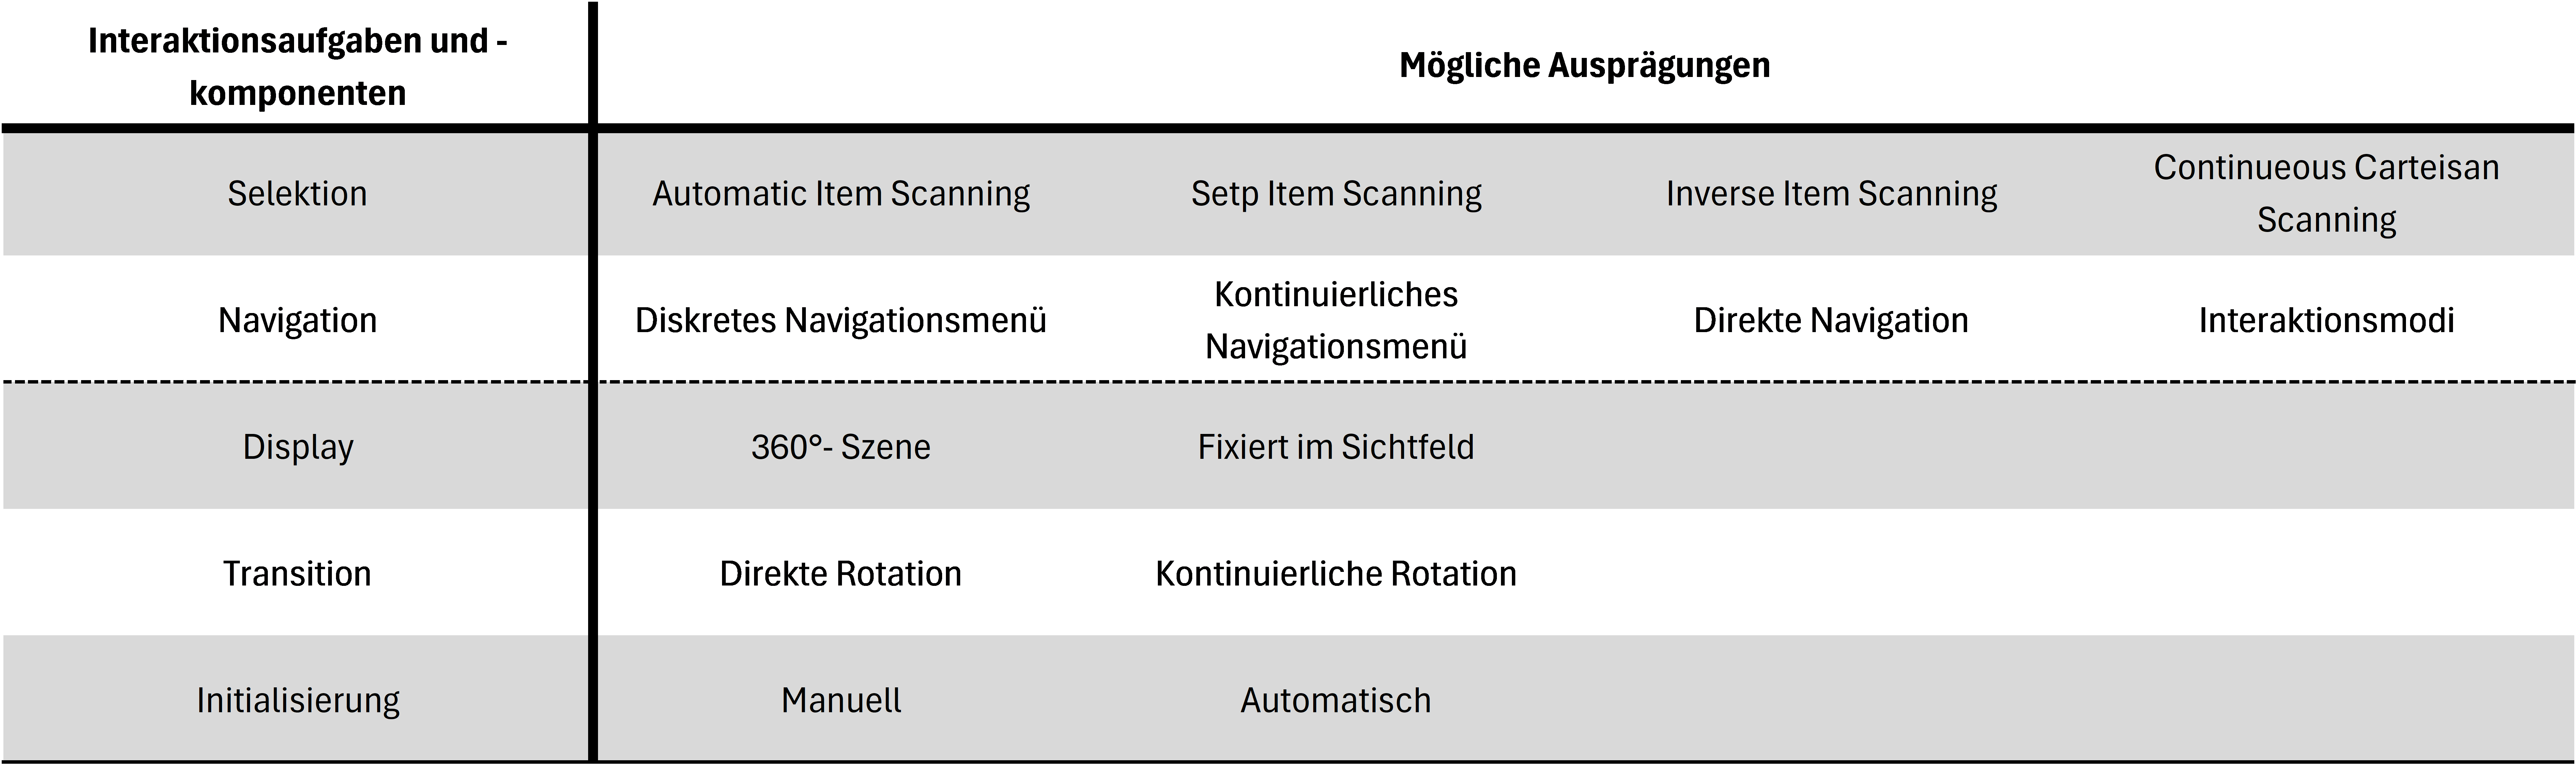
\includegraphics[width=0.95\textwidth]{images/MorphKasten-Ausgang.png}
    \caption{Darstellung der möglichen Ausprägungen der Interaktionsaufgaben und -komponenten}
    \label{fig:MorphKasten-Leer}
\end{figure}

\section{Einordnung und Bewertung der Interaktionsaufgaben und Komponenten anhand der Parameter}
\label{subchap:EinordnungNachParameter}

In diesem Abschnitt werden die zuvor beschriebenen Gestaltungsoptionen der Interaktionsaufgaben und -komponenten systematisch anhand der definierten Parameter bewertet und eingeordnet. Durch soll eine fundierte Grundlage für die Auswahl der finalen Konzepte geschaffen werden. Diese Einschätzung basiert auf den Erkenntnissen der Literatur sowie einer Analyse der vorgestellten Optionen. Es ist jedoch wichtig zu betonen, dass nicht alle Bewertungen durch empirische Daten belegt oder validiert sind, sondern auf einer fundierten, jedoch subjektiven Einschätzung beruhen. 

{\normalfont \bfseries Interaktionsaufgaben}  

\textbf{1. Selektion}

Im Folgenden erfolgt die Einordnung der für die Selektion erarbeiteten Gestaltungsoptionen anhand der definierten Parameter. Dabei wird jeder Parameter einzeln betrachtet, um die spezifischen Stärken und Schwächen der Optionen detailliert zu analysieren. Die Ergebnisse werden in \autoref{fig:Netz-Selektion} visualisiert und bieten eine zusammenfassende Darstellung der Parameterbewertungen.

\begin{figure}[tbh]
    \centering
    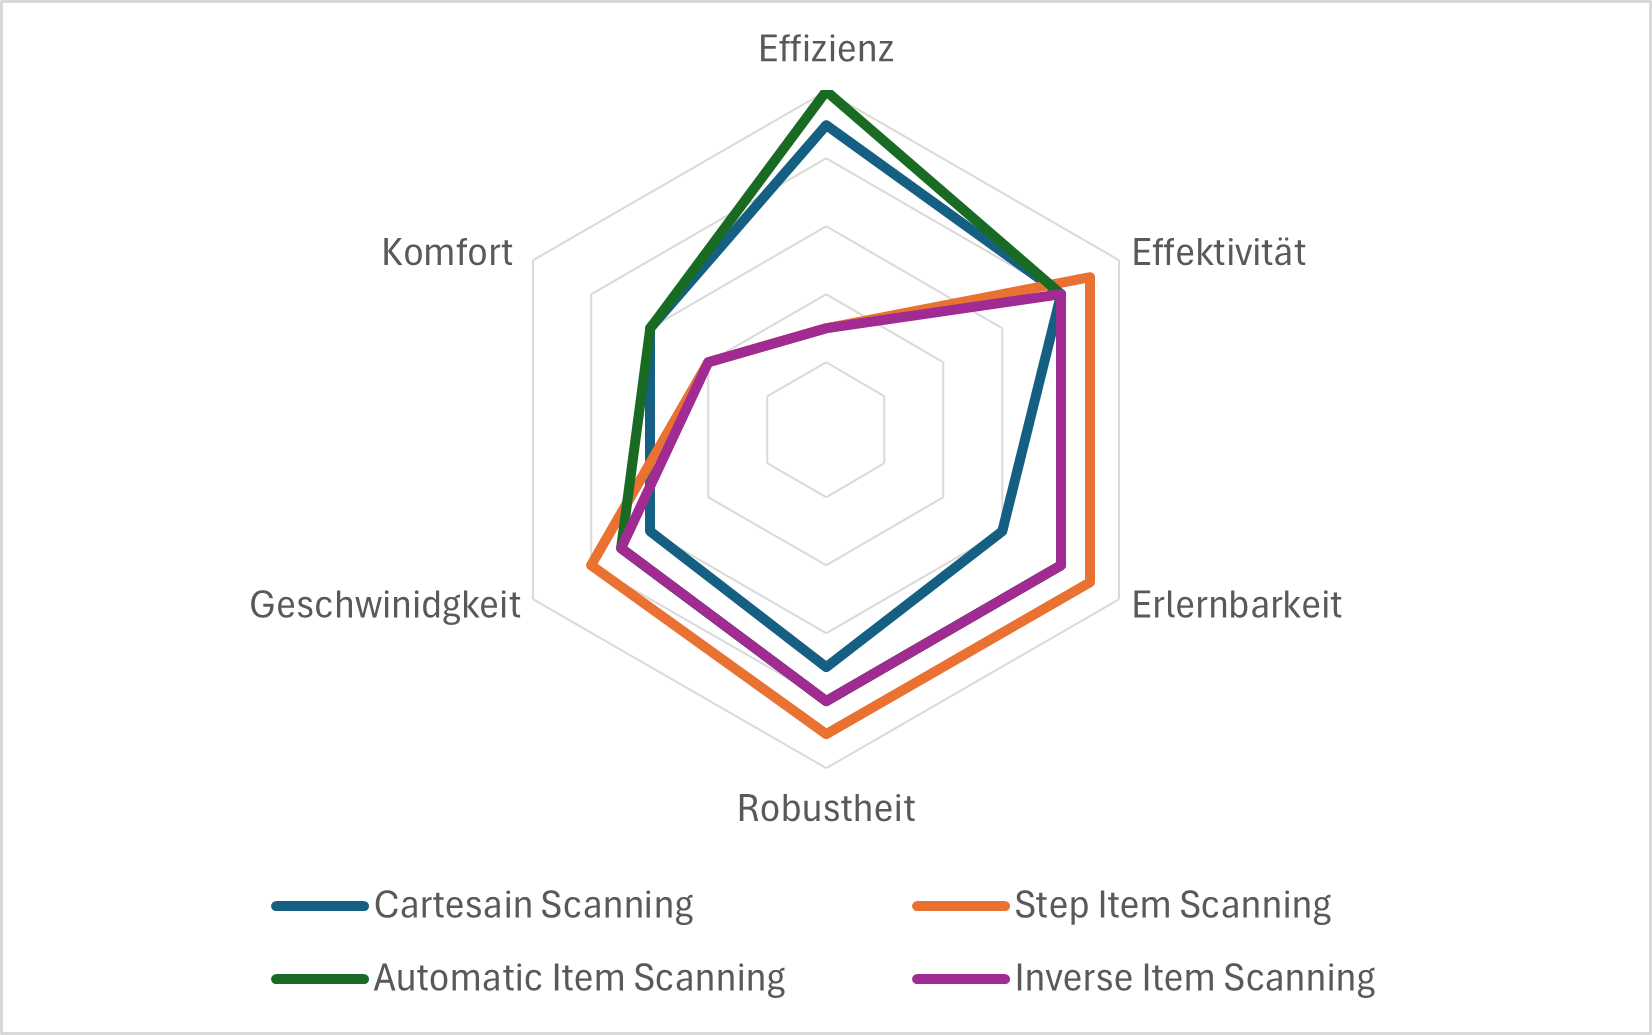
\includegraphics[width=0.75\textwidth]{images/Netzdiagramm-Selektion.png}
    \caption{Visualisierung der Einordnung der Gestaltungsoptionen der Interaktionsaufgabe Selektion}
    \label{fig:Netz-Selektion}
\end{figure}

\textit{Effizienz:}
Ein effizientes binäres Selektionsverfahren sollte eine geringe Anzahl von Schalterbetätigungen und einen möglichst geringen physischen Aufwand für die Interaktion erfordern. Die verschiedenen Auswahlverfahren unterscheiden sich in dieser Hinsicht deutlich. Cartesian Scanning erfordert zwei Schalteraktivierungen, um eine Interaktion durchzuführen. Die klare Struktur und die relativ geringe Anzahl an Aktivierungen ermöglichen eine gute Effizienz.. Automatic Item Scanning zeichnet sich durch eine besonders geringe Anzahl von Aktivierungen aus, da die Selektion eines Elements in der Regel durch eine einzige Schalteraktivierung erfolgt. Dies macht die Methode besonders effizient. Wird allerdings eine Gruppierung von Elementen zur Beschleunigung der Interaktionsgeschwindigkeit eingesetzt, wirkt sich dies leicht negativ auf die Effizienz aus, da die Anzahl der erforderlichen Aktivierungen steigt. Step Item Scanning zeigt eine Effizienz, die stark von der Anzahl der Elemente in der Szene abhängt. Bei einer großen Anzahl von Elementen benötigt das Verfahren entsprechend viele Aktivierungen, um ein Ziel zu erreichen, was die Effizienz deutlich verringert. Eine Gruppierung der Elemente kann jedoch die Effizienz in Szenen mit vielen Elementen erhöhen, da weniger Schritte notwendig sind, um eine Auswahl zu treffen. Auch in Szenarien mit wenigen Elementen ist der Aufwand höher als bei Cartesian Scanning oder Automatic Item Scanning. Inverse Item Scanning ist ebenfalls stark von der Anzahl der Elemente in der Szene abhängig. Je mehr Elemente vorhanden sind, desto länger muss der Schalter gehalten werden, um das gewünschte Zielobjekt zu erreichen. Dies führt zu einem proportionalen Anstieg der körperlichen Anstrengung und verringert die Effizienz in Szenen mit vielen Elementen. Bei wenigen Elementen ist der Aufwand entsprechend geringer. Dennoch bleibt das kontinuierliche Halten des Schalters eine körperlich anstrengendere Interaktionsform. 

\textit{Effektivität:}
Die Effektivität beschreibt, wie zuverlässig und präzise ein gewünschtes Interaktionselement ausgewählt werden kann. Das Cartesian Scanning erfordert präzises Timing, da der Nutzende den Schnittpunkt der Linien im richtigen Moment setzen muss. Ein Verfehlen des Zielobjekts ist möglich, insbesondere bei geringer Übung oder hohen Geschwindigkeiten des Scannings. Das Cartesian Scanning ermöglicht jedoch eine sehr präzise Selektion, insbesondere mit etwas Erfahrung. 
Das Automatic Item Scanning erzielt eine leicht höhere Effektivität. Da nur interaktive Elemente selektiert werden können, sind Fehlselektionen weniger wahrscheinlich. Dennoch spielt auch hier das Timing eine wesentliche Rolle, da das gewünschte Element verpasst werden kann, wenn die Aktivierung nicht rechtzeitig erfolgt. Das Step Item Scanning wird als das effektivste Verfahren eingeschätzt. Die Nutzenden haben die volle Kontrolle über die Auswahl und können in ihrem eigenen Tempo navigieren. Dies minimiert die Wahrscheinlichkeit von Fehlselektionen und gibt ihnen mehr Sicherheit, insbesondere in komplexen Szenarien mit vielen Elementen. Das Inverse Item Scanning zeigt eine Effektivität, die mit der des Automatic Item Scannings vergleichbar ist. Auch hier ist das Timing entscheidend, da der Schalter zum richtigen Zeitpunkt losgelassen werden muss, um das gewünschte Ziel zu erreichen. Die Möglichkeit von Fehlselektionen durch ungenaues Timing ist ein potenzieller Nachteil \citep{COOK2015117}.

\textit{Erlernbarkeit:}
Die Erlernbarkeit beschreibt, wie schnell und intuitiv ein Scanning-Verfahren von den Nutzenden verstanden und angewendet werden kann. Das Step Item Scanning weist die höchste Erlernbarkeit auf. Es ermöglicht den Nutzenden die größte Kontrolle über das Scanning, da sie in ihrem eigenen Tempo navigieren können. Diese direkte Steuerbarkeit reduziert die kognitiven und sensorischen Anforderungen \citep{cook_chapter_2015}, was sich positiv auf das Verständnis der Funktionsweise auswirken könnte. Automatic Item Scanning und Inverse Item Scanning sind in ihrer Erlernbarkeit vergleichbar. Beide Verfahren erfordern die Fähigkeit, das richtige Timing zu finden, um das gewünschte Element auszuwählen. Cartesian Scanning wird als das herausforderndste Verfahren eingestuft. Hier müssen die Nutzenden sowohl der horizontalen als auch der vertikalen Bewegung der Scan-Linien folgen, was ein höheres Maß an Aufmerksamkeit erfordert. Darüber hinaus sind genauere Eingaben erforderlich. Insbesondere für Personen, die mit Scanning-Verfahren weniger vertraut sind, könnte dies anfangs zu Schwierigkeiten führen.
Insgesamt dürften Personen mit Vorerfahrung im Umgang mit Schaltersteuerungen alle beschriebenen Verfahren als vertraut wahrnehmen. Scanning-Verfahren sind aus gängigen Betriebssystemen bekannt (z. B. \citep{apple_einfuhrung_2024, Google-Switch-Access}), was die Erlernbarkeit für diese Zielgruppe deutlich erleichtern kann.

\textit{Robustheit:}
Die Robustheit beschreibt, wie zuverlässig ein Scanning-Verfahren funktioniert und das Auftreten von Fehlern vermeidet. Die Festlegung einer geeigneten Scan-Rate ist ein wesentlicher Faktor für die Robustheit von Scanning-Verfahren. Eine zu hohe Scan-Rate kann dazu führen, dass den Nutzenden nicht ausreichend Zeit zur Verfügung steht, um eine präzise Selektion durchzuführen \citep{COOK2015117}. Dieses Problem betrifft insbesondere das Cartesian Scanning sowie das Automatic und Inverse Item Scanning. Das Step Item Scanning hingegen wird als das robusteste Verfahren eingestuft, da die Nutzenden die Scan-Rate jederzeit selbst steuern können. Fehler, die aus einer zu schnellen oder zu langsamen Scan-Rate resultieren, können so vermieden werden. Diese Steuerbarkeit stellt sicher, dass das Verfahren flexibel auf unterschiedliche Anforderungen der Nutzenden ausgerichtet werden kann \citep{COOK2015117}.
Das Automatic Item Scanning und das Inverse Item Scanning weisen eine etwas geringere Robustheit auf. Beide Verfahren sind stark von einer geeigneten Einstellung der Scan-Rate abhängig, da die Nutzenden das Timing der Selektion genau treffen müssen. Zudem können bei beiden Verfahren Fehler auftreten, wenn die Reihenfolge der Elemente nicht intuitiv gestaltet ist. Um dem entgegenzuwirken, sollte die Reihenfolge der Elemente möglichst nachvollziehbar gestaltet werden und eine klare Visualisierung gewählt werden, die bereits Hinweise auf das jeweils nächste Element in der Scan-Reihenfolge gibt.
Das Cartesian Scanning wird mit einer mittleren Robustheit bewertet. Auch hier kann eine unpassende Scan-Rate die Präzision der Selektion beeinträchtigen. Außerdem besteht das Risiko, dass kleine Ungenauigkeiten beim Setzen der Scan-Linien zu unerwünschten Ergebnissen führen. Um die Robustheit zu erhöhen, könnte ein Toleranzbereich implementiert werden, der kleinere Ungenauigkeiten toleriert und damit die Intentionen der Nutzenden besser interpretiert. Die Interpretation der Intention von Eingaben stellt gemäß \citet{dombrowski_designing_2019} generell eine Maßnahme dar, um Barrieren bei der Nutzung von VR abzubauen. 

\textit{Interaktionsgeschwindigkeit:}
Im Vergleich zu direkten Interaktionsmethoden weisen Scanning-Verfahren generell eine langsamere Interaktionsgeschwindigkeit auf \citep{COOK2015117}. Die folgende Bewertung bezieht sich daher ausschließlich auf den relativen Vergleich der verschiedenen Scanning-Methoden untereinander. 
Ein wesentlicher Einflussfaktor auf die Interaktionsgeschwindigkeit beim Item Scanning ist die Anzahl der Interaktionselemente in der Szene, da ein sequentieller Durchlauf aller Interaktionselemente erfolgt \cite{10.1145/2159365.2159386}. Mit zunehmender Anzahl der Elemente steigt daher die Wahrscheinlichkeit, dass sich das Zielobjekt weiter hinten in der Scan-Reihenfolge befindet, was die Interaktionsgeschwindigkeit deutlich reduziert. Eine Maßnahme, um diesem Umstand entgegenzuwirken, besteht in der Gruppierung räumlich oder semantisch zusammenliegender Elemente. Die Geschwindigkeit des Item Scannings lässt sich dadurch deutlich erhöhen \citep{COOK2015117}. In Szenen mit wenigen Elementen oder wenn sich das Zielobjekt weiter vorne in der Sequenz befindet, kann hingegen eine höhere Interaktionsgeschwindigkeit erreicht werden. Das Step Item Scanning bietet gegenüber dem Automatic und Inverse Item Scanning den Vorteil, dass die Nutzenden den Scan-Vorgang aktiv steuern und direkt zum gewünschten Zielobjekt navigieren können, wodurch längere Wartezeiten vermieden werden. Dementsprechend wird die Interaktionsgeschwindigkeit des Automatic und Inverse Item Scanning als moderat bewertet, während das Step Item Scanning eine höhere Interaktionsgeschwindigkeit aufweist.
Das Cartesian Scanning hingegen weist eine konstantere Interaktionsgeschwindigkeit auf, da die Anzahl der Elemente in der Szene keinen direkten Einfluss auf die Dauer des Scan-Vorgangs hat. Es besteht jedoch ein Zusammenhang zwischen der Interaktionsgeschwindigkeit und der Position des Zielobjekts in der Szene. Befindet sich das Objekt weiter entfernt vom Startpunkt der Scan-Linien, kann es zu Verzögerungen kommen, bis die Linien das gewünschte Element erreichen. Die Stärke dieses Effekts ist jedoch noch unklar und bedarf weiterer Untersuchungen. Insgesamt wird die Interaktionsgeschwindigkeit des Cartesian Scanning als moderat eingestuft.

\textit{Komfort:} 
Beim Komfort von Scanning-Verfahren ist insbesondere die Wahrscheinlichkeit des Auftretens motorischer Ermüdung sowie der kognitiven und visuellen Anstrengung zu berücksichtigen.
Cartesian Scanning erfordert nur wenige Aktivierungen des Schalters, was das Risiko motorischer Ermüdung vergleichsweise gering hält. Allerdings erfordert das Verfahren ein präzises Timing sowie eine erhöhte visuelle Aufmerksamkeit, da die Bewegung der Scan-Linien kontinuierlich verfolgt werden muss. Dies führt zu einer erhöhten kognitiven Beanspruchung. Das Automatic Item Scanning zeichnet sich ebenfalls durch eine geringe Anzahl erforderlicher Schalteraktivierungen aus, wodurch die motorische Belastung begrenzt bleibt. Allerdings erfordert das Verfahren eine hohe visuelle Aufmerksamkeit und ein exaktes Timing, was die Anforderungen an die Konzentration erhöht. Das Step Item Scanning erfordert eine deutlich höhere Anzahl an Aktivierungen, was zu einer höheren motorischen Belastung und einem erhöhten Risiko der motorischen Ermüdung führt. Gleichzeitig ist die Anforderung an die visuelle Aufmerksamkeit geringer, da weder ein genaues Timing noch ein kontinuierliches Verfolgen des Scans erforderlich ist und die Nutzenden mehr Kontrolle über den Scan-Vorgang haben. Dadurch wird die kognitive Belastung reduziert. Dennoch wird der Komfort des Step Item Scanning aufgrund der hohen motorischen Anforderungen als gering bewertet. Inverse Item Scanning liegt hinsichtlich der motorischen Belastung zwischen Automatic und Step Item Scanning. Das Halten des Schalters erfordert eine moderate körperliche Anstrengung, die höher als beim Automatic Item Scanning, aber geringer als beim Step Item Scanning ist. Außerdem ist eine erhöhte visuelle Aufmerksamkeit erforderlich, um das Timing präzise zu steuern. Der Komfort des Inverse Item Scanning wird daher ebenfalls als gering bewertet \citep{COOK2015117}.

\textbf{2. Navigation} 

Im Folgenden erfolgt die Einordnung der für die Navigation erarbeiteten Gestaltungsoptionen anhand der definierten Parameter. Die Ergebnisse aus dieser Einordnung werden in \autoref{fig:Netz-Navigation} zusammenfassend visualisiert. 

\begin{figure}[tbh]
    \centering
    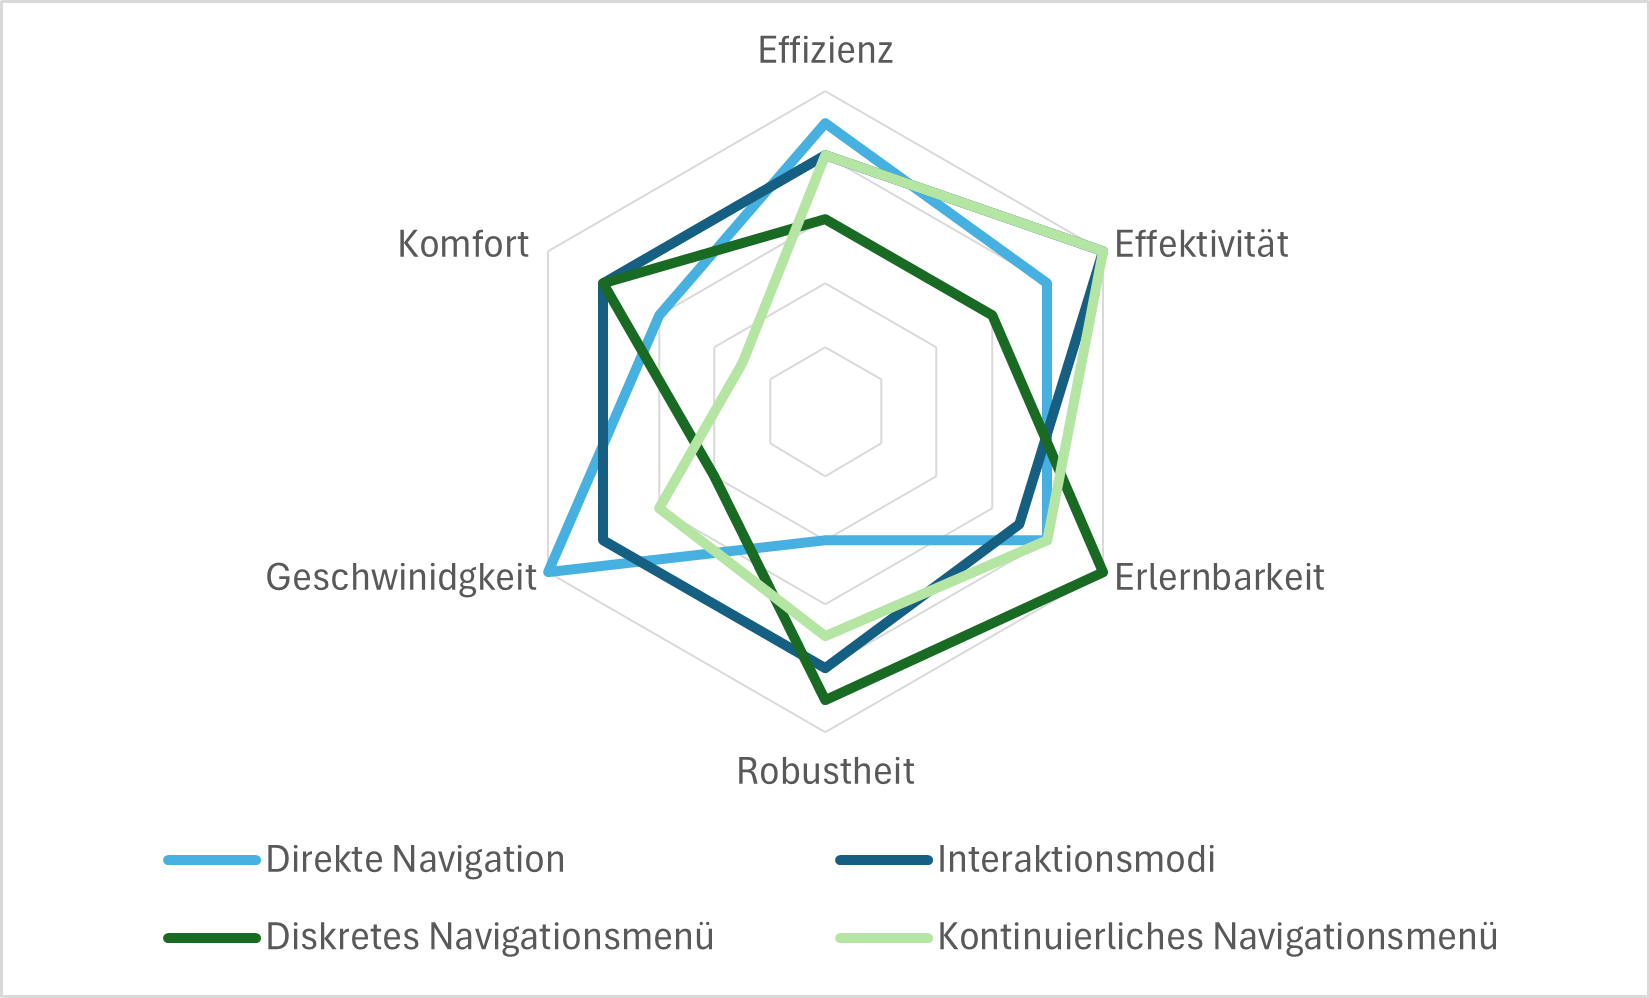
\includegraphics[width=0.75\textwidth]{images/Netzdiagramm-Navigation.png}
    \caption{Visualisierung der Einordnung der Gestaltungsoptionen der Interaktionsaufgabe Navigation}
    \label{fig:Netz-Navigation}
\end{figure}

\textit{Effizienz:}
Die Effizienz der Gestaltungsoptionen der Navigation wird durch den erforderlichen Interaktionsaufwand bestimmt. Der Schwerpunkt liegt hier auf der Anzahl der Eingaben, die zur Durchführung der Navigation erforderlich sind. Die beiden auf dem Cartesian Scanning basierenden Optionen weisen unterschiedliche Effizienzniveaus auf. Die direkte Navigation erfordert lediglich die Festlegung des Schnittpunktes, was eine relativ hohe Effizienz gewährleistet. Allerdings steigt der Interaktionsaufwand bei größeren Rotationswinkeln, da in diesen Fällen mehrere Navigationsschritte erforderlich sein können, um den gewünschten Endpunkt zu erreichen. Die Navigation mit separaten Interaktionsmodi erfordert zusätzlich eine Interaktion, um den Moduswechsel zwischen Navigation und Selektion durchzuführen, was den Aufwand geringfügig erhöht. Daher wird die Effizienz der direkten Navigation etwas höher eingeordnet. 
Bei den Optionen des Item-Scannings hat der gewünschte Rotationswinkel einen erheblichen Einfluss auf die Effizienz. Bei der diskreten Navigation führt ein größerer Winkel zu einer höheren Anzahl von Eingaben, da die Rotation in festen Schritten erfolgt. Dies macht die Methode bei großen Rotationswinkeln weniger effizient. Dagegen erfordert die kontinuierliche Navigation bei kleinen Rotationen einen geringfügig höheren Aufwand, da zwei Eingaben erforderlich sind (eine zum Aktivieren und eine zum Beenden der Navigation). Dieser Mehraufwand wird jedoch bei großen Rotationswinkeln durch die Möglichkeit der kontinuierlichen Navigation kompensiert. Die Effizienz der diskreten Navigation als etwas geringer eingestuft.

\textit{Effektivität:}
Die Effektivität der Gestaltungsoptionen der Navigation wird durch die Genauigkeit bestimmt, mit der ein gewünschter Rotationswinkel erreicht werden kann. Dabei wird insbesondere berücksichtigt, inwieweit die Nutzenden die Navigation kontrollieren und den Rotationswinkel exakt bestimmen können. 
Ein deutlicher Unterschied in der Effektivität zeigt sich bei den Optionen, die auf dem Cartesian Scanning basieren. Die direkte Navigation wird durch die Position und Anzahl der Interaktionselemente in der Szene eingeschränkt. Je mehr Elemente vorhanden sind, desto mehr leidet die Effektivität, da nur Punkte im Raum ausgewählt werden können, an denen sich kein Interaktionselement befindet. Dies schränkt die Kontrolle über den Rotationswinkel erheblich ein. Bei Szenen mit wenigen Interaktionselementen ist dieser Effekt jedoch praktisch vernachlässigbar. Die Navigation mit Interaktionsmodi bietet hingegen eine deutlich höhere Flexibilität, da beliebige Rotationswinkel erreicht werden können.
Auch die Optionen des Item-Scannings unterscheiden sich in ihrer Effektivität. Das Navigationsmenü mit diskreter Rotation erlaubt nur eine begrenzte Anzahl von vorgegebenen Rotationswinkeln. Dies führt dazu, dass die Zielposition nicht immer exakt erreicht werden kann, was wiederum die Effektivität einschränkt. Im Gegensatz dazu bietet die kontinuierliche Rotation durch ihre Flexibilität die Möglichkeit, jeden beliebigen Winkel zu erreichen. Diese Methode gewährleistet somit eine hohe Präzision \citep{10.1145/2159365.2159386}. 

\textit{Erlernbarkeit:} 
Bei der direkten Navigation beim Cartesian Scanning profitieren die Nutzenden von der Vertrautheit mit dem Prinzip aus der Selektion, sodass keine neuen Mechanismen erlernt werden müssen. Allerdings kann die Durchführung der Navigation aufgrund der notwendigen Koordination zwischen Selektion und Navigation anfangs eine gewisse Herausforderung darstellen. Insgesamt wird die Erlernbarkeit daher als hoch eingeschätzt. Die Interaktionsmodi erfordern zusätzlich das Verständnis, wann welcher Modus aktiv ist und wie zwischen den Modi gewechselt wird. Dies könnte eine leichte kognitive Hürde darstellen, insbesondere wenn der Moduswechsel eine andere Art der Eingabe als die Selektion erfordert (z. B. Halten des Schalters oder zwei schnelle Aktivierungen hintereinander). Während das zugrundeliegende Konzept einfach ist, kann die anfängliche Anwendung für neue Benutzer anspruchsvoller sein. Die Erlernbarkeit wird daher als moderat bewertet.
Die diskrete Navigation im Navigationsmenü basiert auf klaren und konsistenten Schritten. Die Nutzenden wählen Buttons aus, die festgelegte Rotationswinkel repräsentieren. Dies macht die Bedienung besonders einfach und einsteigerfreundlich, da keine zusätzlichen Mechanismen erlernt werden müssen. Durch die intuitive Interaktionslogik wird die Erlernbarkeit als sehr hoch bewertet.
Die kontinuierliche Navigation ermöglicht es, die Rotation durch einmalige Selektion eines Buttons zu starten und durch erneute Selektion desselben Buttons zu stoppen. Dieser Mechanismus ist prinzipiell leicht verständlich, kann aber anfangs nicht ganz intuitiv sein, da den Nutzenden möglicherweise nicht klar ist, wie die Rotation wieder gestoppt werden kann. Aufgrund dieser geringen Einstiegshürde wird die Erlernbarkeit als hoch eingeschätzt.

\textit{Robustheit:}
Bei der direkten Navigation (basierend auf dem Cartesain Scanning) können Fehler durch fehlende Abgrenzung zwischen Selektion und Navigation entstehen. Insbesondere in Szenen mit vielen Interaktionselementen oder bei ungenauem Timing kann es zu Verwechslungen kommen, etwa wenn Nutzende ein Element selektieren möchten, die Eingabe jedoch knapp verfehlen. Dies kann dazu führen, dass stattdessen eine Navigation ausgelöst wird, was die Robustheit maßgeblich beeinträchtigt. Die Einführung eines separaten Modus für Navigation und Selektion hingegen minimiert die Wahrscheinlichkeit solcher Fehler und erhöht die Robustheit deutlich. Dennoch können Fehler auftreten, wenn versehentlich der falsche Modus aktiv ist. Bspw. könnte eine Selektion gewünscht sein, während der Navigationsmodus noch aktiv ist. Solche Situationen erfordern eine bewusste Kontrolle durch die Nutzenden, um zwischen den Modi zu wechseln. Insgesamt wird die Robustheit der Interaktionsmodi jedoch als deutlich höher eingeschätzt als die der direkten Navigation.
Ein Navigationsmenü bietet in beiden Varianten eine robuste Kontrolle über die Navigation. Jedoch können Timing-Probleme dazu führen, dass versehentlich in die falsche Richtung navigiert wird. Solche Fehler lassen sich in beiden Varianten korrigieren, jedoch unterscheidet sich der Aufwand je nach Mechanismus. Bei der diskreten Navigation führt eine Fehleingabe lediglich zu einem einzelnen Schritt in die falsche Richtung. Der Fehler kann leicht korrigiert werden, indem im Anschluss die entgegengesetzte Richtung gewählt wird. Die kontinuierliche Navigation erfordert hingegen mehr Aufwand für die Fehlerkorrektur. Nutzende müssen zunächst die aktive Eingabe abbrechen, anschließend die Eingabe für die eigentlich gewünschte Richtung aktivieren und diese wiederum abbrechen, sobald die Korrektur abgeschlossen ist. Dies führt zu einem erhöhten Zeit- und Arbeitsaufwand, was die Robustheit des Verfahrens im Vergleich zur diskreten Navigation verringert \citep{10.1145/2159365.2159386}. 

\textit{Interaktionsgeschwindigkeit:}
Die direkte Navigation wird als die schnellste Option angesehen. Da keine zusätzlichen Schritte für den Wechsel zwischen Selektion und Navigation notwendig sind, kann die Navigation unmittelbar durchgeführt werden. Darüber hinaus ermöglicht die direkte Navigation, einen großen Rotationswinkel mit nur einer Navigation zu erreichen, indem der Schnittpunkt bswp. weit an den Rand des aktuellen Sichtfeldes gesetzt wird. Dies reduziert die Anzahl der notwendigen Navigationen und erhöht damit die Interaktionsgeschwindigkeit. Einschränkungen können jedoch auftreten, wenn die Anzahl oder Position der Interaktionselemente in der Szene die Wahl eines großen Winkels verhindert. Die Option mit getrennten Interaktionsmodi erfordert einen Zwischenschritt, da zwischen Selektion und Navigation gewechselt werden muss, was zusätzliche Zeit in Anspruch nimmt. Nach dem Moduswechsel bietet die Navigation jedoch die gleichen Vorteile wie die direkte Navigation. Darüber hinaus bestehen hier keine Einschränkungen hinsichtlich der Anzahl oder Position der Elemente. 
Die Navigation über ein Navigationsmenü erfordert zunächst das Öffnen des Menüs, was einen Zwischenschritt darstellt, der sich negativ auf die Geschwindigkeit auswirkt. Bei der diskreten Navigation wird die Geschwindigkeit zusätzlich durch die Anzahl der erforderlichen Schritte beeinflusst. Um eine größere Rotation zu erreichen, müssen mehrere Interaktionen nacheinander ausgeführt werden. Dies führt zu einer insgesamt geringeren Geschwindigkeit, insbesondere bei größeren Rotationswinkeln. Im Vergleich zur diskreten Variante ist die kontinuierliche Navigation schneller \citep{10.1145/2159365.2159386}, da eine kontinuierliche Rotation gestartet werden kann, die nur durch eine weitere Interaktion gestoppt werden muss. Dies reduziert die Anzahl der notwendigen Interaktionen und beschleunigt die Navigation insbesondere bei größeren Rotationswinkeln. Jedoch wirkt sich auch hier der Zwischenschritt des Öffnens des Menüs negativ auf die Geschwindigkeit aus. 

\textit{Komfort:}
Der Komfort der Navigation wird maßgeblich durch die erforderliche Konzentration, den allgemeinen kognitiven Aufwand sowie den visuellen Anspruch beeinflusst. Die Optionen, die auf dem Cartesian Scanning basieren, erfordern insgesamt eine präzise Auswahl, um den gewünschten Rotationspunkt zu erreichen. Diese Präzision geht mit einer leicht erhöhten Konzentration einher. Bei der direkten Navigation ist zusätzlich zu berücksichtigen, dass eine unbeabsichtigte Auswahl eines Interaktionselements möglich ist, was den kognitiven Aufwand weiter erhöht. Die Interaktionsmodi-Option reduziert das Risiko von Fehleingaben durch die Trennung von Selektion und Navigation. Dies führt zu einer leicht reduzierten kognitiven Belastung im Vergleich zur direkten Navigation. Die visuelle Komplexität der Szene wird durch das Hinzufügen zusätzlichenr Interaktionselemente für das Navigationsmenü leicht erhöht. Die diskrete Navigation mit vorgegebenen Rotationswinkeln erfordert insgesamt die geringste Konzentration, da die Interaktion sehr konsistent ist. Dadurch wird die kognitive Belastung minimiert.
Die kontinuierliche Navigation benötigt ein gewisses Timing, um die Rotation im gewünschten Moment zu stoppen. Dies erfordert eine erhöhte Konzentration im Vergleich zur diskreten Option. Darüber hinaus besteht bei einer durchgängigen Rotation der First-Person-Kamera ein erhöhtes Risiko für Motion Sickness, was den Komfort weiter beeinträchtigen kann \citep{10.1007/s10055-020-00425-x, 8797722}.


{\normalfont \bfseries Interaktionskomponenten:} 

\textbf{1. Display}

Folgend werden die erarbeiteten Gestaltungsoptionen für die Komponente Display anhand der definierten Parameter eingeordnet. Die Ergebnisse dieser Einordnung sind in \autoref{fig:Netz-Display} zusammenfassend visualisiert.

\begin{figure}[tbh]
    \centering
    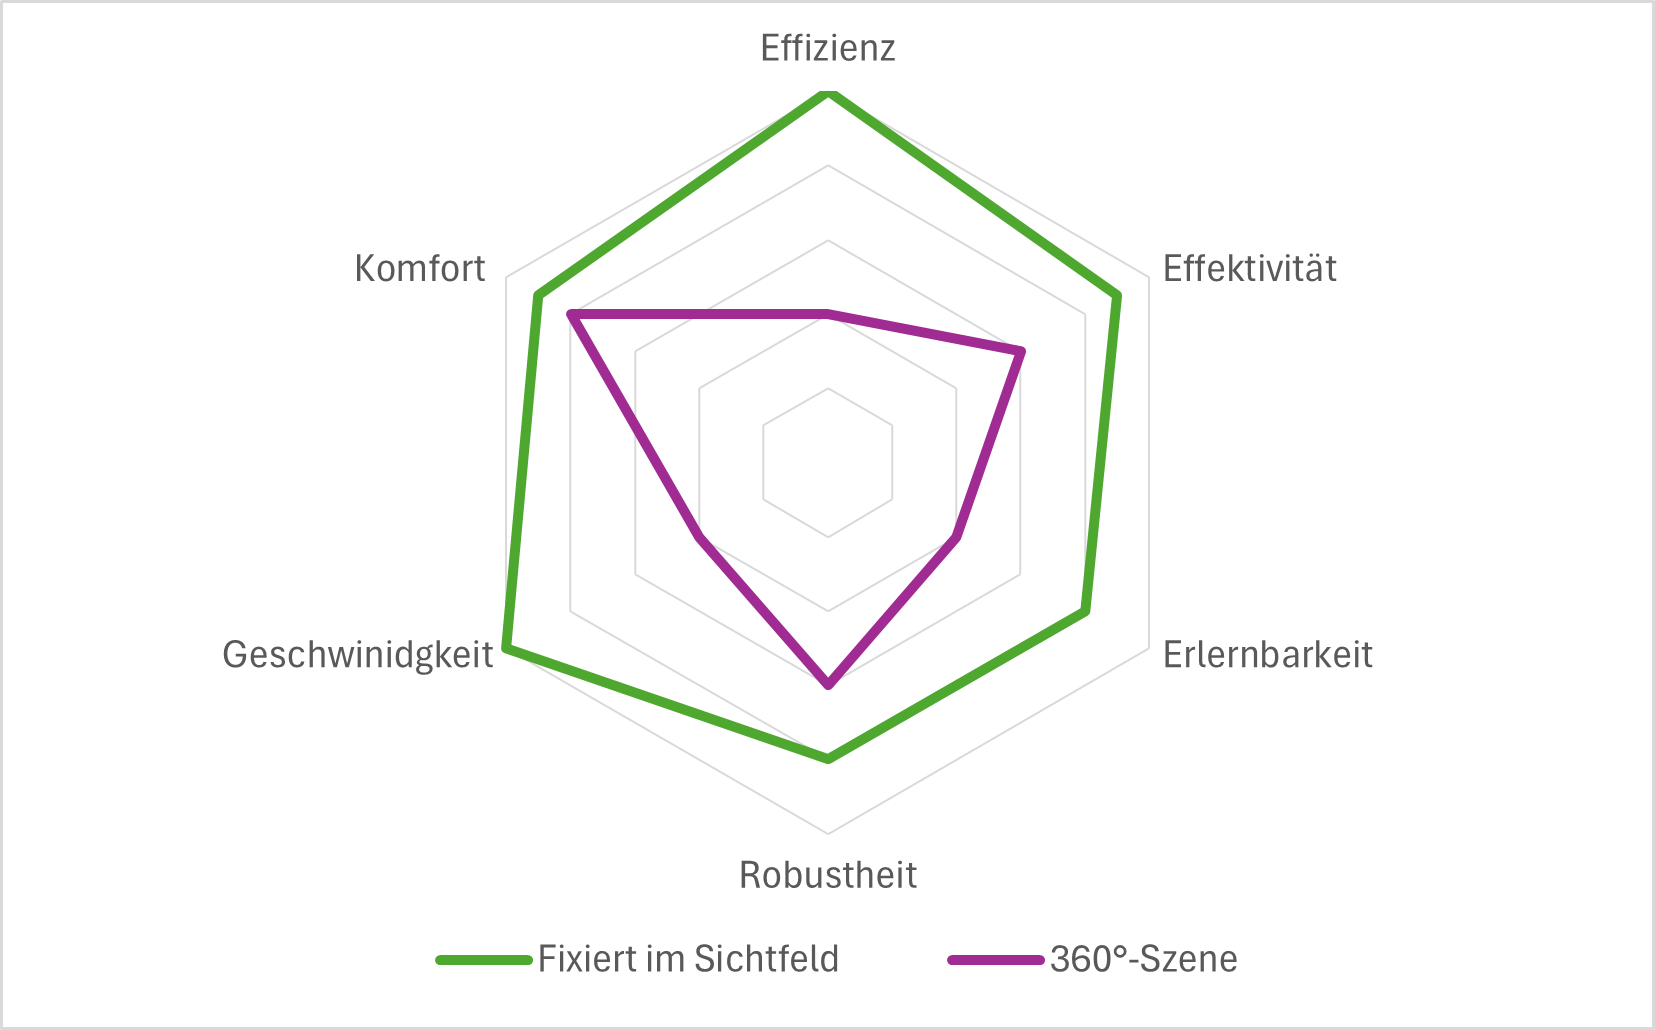
\includegraphics[width=0.75\textwidth]{images/Netzdiagramm-Display.png}
    \caption{Visualisierung der Einordnung der Gestaltungsoptionen der Interaktionskomponente Display}
    \label{fig:Netz-Display}
\end{figure}

\textit{Effizienz:}
Die Effizienz der verschiedenen Optionen zur Darstellung des Scanning-Verfahrens in der virtuellen Umgebung wird hinsichtlich des erforderlichen Aufwands analysiert. Es zeigt sich, dass der Einfluss der Display-Optionen von der Art des Scanning-Verfahrens abhängt.
Sowohl beim Automatic Item Scanning als auch beim Cartesain Scanning ist der Aufwand unabhängig davon, ob das Scanning-Verfahren auf das Sichtfeld beschränkt oder auf die gesamte Szene ausgeweitet wird. Bei beiden Verfahren erfolgt das Scanning automatisiert und die präsentierte Auswahl (Item: hervorgehobenes Element, Cartesain: Position der Linien) wird durch Aktivierung des Schalters ausgewählt. Im Gegensatz dazu zeigt sich bei Step und Inverse Item Scanning ein deutlicher Einfluss der Display-Optionen. Wird das Scanning auf die gesamte Szene ausgeweitet, werden alle Interaktionselemente unabhängig von ihrer Position in das Scan-Set einbezogen. Dadurch erhöht sich die Anzahl der zu durchlaufenden Elemente. Beim Step Item Scanning erhöht sich dadurch die Anzahl der erforderlichen Schalterbetätigungen und beim Inverse Item Scanning wird ein längeres Halten des Schalters erforderlich. Dies führt zu einem deutlich erhöhten Aufwand und damit zu einer geringen Effizienz. Eine Beschränkung des Scan-Sets auf Elemente im Sichtfeld hingegen reduziert die Anzahl der zu durchlaufenden Interaktionselemente und damit den erforderlichen Aufwand bei beiden Verfahren deutlich. Dies ist insbesondere bei Szenen mit vielen Interaktionselementen entscheidend. 

\textit{Effektivität:}
Die Fixierung des Scanning-Verfahren an das Sichtfeld des Nutzenden ermöglicht eine feinere Kontrolle des Scanning, da der Scan-Bereich immer visuell verfolgt werden kann, was sich wiederum positiv auf die Effektivität auswirkt. Ist das Scanning-Verfahren auf die gesamte Szene ausgeweitet, tritt der gegenteilige Effekt ein. In diesem Fall wird eine präzise Steuerung erschwert, da der Scan-Bereich nicht vollständig visuell erfasst werden kann, was insbesondere bei komplexen Szenen zu Verwirrung und damit zu unpräziseren Interaktionen führen kann. Die Effektivität wird daher für die Fixierung als hoch bewertet und für die Ausweitung auf den gesamten 360°-Bereich der Szene als moderat. 

\textit{Erlernbarkeit:} 
Bei der Fixierung im Sichtfeld bleibt der gesamte Scan-Vorgang im sichtbaren Bereich, was das visuelle Feedback erleichtert. Die Nutzenden können jederzeit erkennen, ob der Scan-Vorgang aktiv ist und diesen verfolgen. Dies erleichtert nicht nur den Einstieg in die Nutzung, sondern reduziert auch das Risiko von Missverständnissen oder Fehleingaben. Im Falle einer Fehleingabe kann diese direkt visuell nachvollzogen und ggf. korrigiert werden. Aufgrund dieser Transparenz wird die Erlernbarkeit dieser Option als hoch bewertet.
Wird das Scanning-Verfahren auf die gesamte Szene ausgeweitet, erfordert dies ein höheres Maß an Verständnis für den Systemzustand, da der Scan-Vorgang auch außerhalb des Sichtfeldes stattfinden kann. Fehlerhafte Schalterbetätigungen können in diesem Fall Systemreaktionen auslösen, die für die Nutzenden nicht unmittelbar nachvollziehbar sind. Dies erschwert das Erlernen und erfordert zusätzliche Rückmeldesysteme, um den Status des Scans verständlich zu machen. Die Erlernbarkeit wird daher als geringer eingestuft. 

\textit{Robustheit:}
Die Fixierung des Scanning-Verfahren auf das Sichtfeld ermöglicht es den Nutzenden, den Scan-Vorgang durch gezielte Kopfbewegungen zu beeinflussen. Diese Möglichkeit kann insbesondere beim Cartesian Scanning die Robustheit erhöhen, da kleinere Ungenauigkeiten durch bewusste Kopfbewegungen korrigiert werden können. Dies setzt allerdings voraus, dass die Nutzenden dazu in der Lage sind, Kopfbewegungen präzise und kontrolliert vorzunehmen. Für Personen mit eingeschränkter motorischer Kontrolle könnte diese Abhängigkeit von der Kopfbewegung unter Umständen problematisch sein und die Robustheit der Interaktion verringern. Unbeabsichtigte Verschiebungen des Scan-Vorgangs durch unkontrollierte Kopfbewegungen oder ungenaue Steuerung können dazu führen, dass Interaktionselemente verfehlt werden. Dies erhöht das Risiko von Navigations- oder Selektionsfehlern. Trotz dieser möglichen Nachteile bleibt die visuelle Rückmeldung innerhalb des Sichtfeldes ein stabilisierender Faktor, der die Nachvollziehbarkeit von Fehlern und deren Korrektur erleichtert. 
Die Integration des Scanning-Verfahren in die gesamte Szene eliminiert die Abhängigkeit von Kopfbewegungen und verhindert somit unbeabsichtigte Verschiebungen des Scannings durch unkontrollierte Bewegungen und erhöht damit die Robustheit des Systems. Diese Option birgt jedoch ein erhöhtes Risiko unbeabsichtigter Selektionen, da der Scan außerhalb des Sichtfeldes stattfinden kann und für die Nutzenden visuell nicht jederzeit nachvollziehbar ist. Bei den Scanning-Verfahren Automatic und Inverse Item Scanning sowie beim Cartesian Scanning können außerdem schneller Timing-Fehler entstehen, wenn der Scan-Vorgang von außerhalb des Sichtfeldes in den Sichtbereich übergeht. In diesem Fall könnte die Reaktionszeit des Nutzenden nicht ausreichen, um das Zielelement rechtzeitig zu selektieren. 

\textit{Interaktionsgeschwindigkeit:}
Die Interaktionsgeschwindigkeit der beiden Display-Optionen unterscheidet sich deutlich. Die Option mit fixiertem Scanning im Sichtfeld bietet deutliche Vorteile in der Interaktionsgeschwindigkeit. Da hier beim Item Scanning nur die Elemente im Sichtfeld gescannt werden, ist die Größe des Scan-Sets begrenzt, was zu einem schnelleren Durchlauf der Sequenz und damit zu einer schnelleren Interaktionsgeschwindigkeit führt. Beim Cartesian Scanning ist die Bewegung der Linien auf einen kleinen Bereich beschränkt, sodass Wartezeiten reduziert werden können. Darüber hinaus können beim Cartesian Scanning Kopfbewegungen (sofern möglich) dazu genutzt werden, die Scan-Linien näher an das gewünschte Zielelement zu bringen, was die Interaktionsgeschwindigkeit beschleunigt. Insgesamt führt die Kombination aus kleiner Größe des Scan-Sets und aktiver Beeinflussbarkeit durch Kopfbewegungen zu einer hohen Interaktionsgeschwindigkeit.
Die auf die gesamte Szene erweiterte Option zeigt eine geringere Interaktionsgeschwindigkeit, insbesondere beim Item Scanning. Da hier alle Elemente der Szene unabhängig von ihrer Position im Sichtfeld berücksichtigt werden, nimmt die Größe des Scan-Sets deutlich zu. Dies führt zu einer Verzögerung, da der Scan-Vorgang mehr Zeit benötigt, um alle Elemente sequentiell zu durchlaufen. Beim Cartesian Scanning ist die Interaktionsgeschwindigkeit ebenfalls niedriger, da die Bewegung der Scan-Linien unabhängig von der Blickrichtung stattfindet und somit mehr Zeit in Anspruch nimmt. Außerdem ist es nicht möglich, den Scan-Vorgang durch Kopfbewegungen gezielt zu beschleunigen. 

\textit{Komfort:}
Der Komfort der beiden Display-Optionen unterscheidet sich deutlich hinsichtlich der erforderlichen Konzentration, der visuellen Komplexität und der motorischen Ermüdung.
Die Fixierung des Scan-Vorgangs im Sichtfeld erfordert ein höheres Maß an Konzentration, da selbst minimale Kopfbewegungen einen direkten Einfluss auf den Scan-Vorgang haben. Dies kann zu ungewollten Verschiebungen führen. Darüber hinaus kann die Kombination von Kopfbewegung und Scanning zu visuellen Irritationen führen, insbesondere wenn die Bewegung der Scan-Linien aufgrund der Kopfbewegung schneller oder unregelmäßiger erscheint. Ein Vorteil dieser Option liegt jedoch in der potenziell geringeren motorischen Ermüdung, da durch die Beschränkung auf das Sichtfeld das Scan-Set verkleinert werden kann, wodurch die Anzahl der erforderlichen Interaktionen reduziert wird, insbesondere bei Verfahren wie Step und Inverse Item Scanning. 
Die Option, das Scanning auf die gesamte 360°-Szene zu erstrecken, bietet hinsichtlich der Konzentration einen deutlichen Vorteil, da Kopfbewegungen keinen Einfluss auf den Scan-Vorgang haben. Dies minimiert die Anforderungen an die Aufmerksamkeit und sorgt für einen gleichmäßigen Ablauf des Scannings, was den Komfort erhöht. Auch die visuelle Komplexität ist vergleichsweise gering, da die Bewegung des Scannings unabhängig von äußeren Einflüssen erfolgt und somit vorhersehbar bleibt. Allerdings zeigt diese Option Schwächen bei der motorischen Ermüdung, insbesondere im Zusammenhang mit Step und Inverse Item Scanning. Die größere Größe des Scan-Sets erfordert eine höhere Anzahl von Interaktionen oder ein längeres Halten des Schalters, was schnell zu Ermüdung führen kann. 

\textbf{2. Transition} 

Im Folgenden erfolgt die Einordnung der erarbeiteten Gestaltungsoptionen für die Komponente Transition anhand der definierten Parameter. Die Ergebnisse dieser Einordnung sind in \autoref{fig:Netz-Transition} zusammenfassend dargestellt. 

\begin{figure}[tbh]
    \centering
    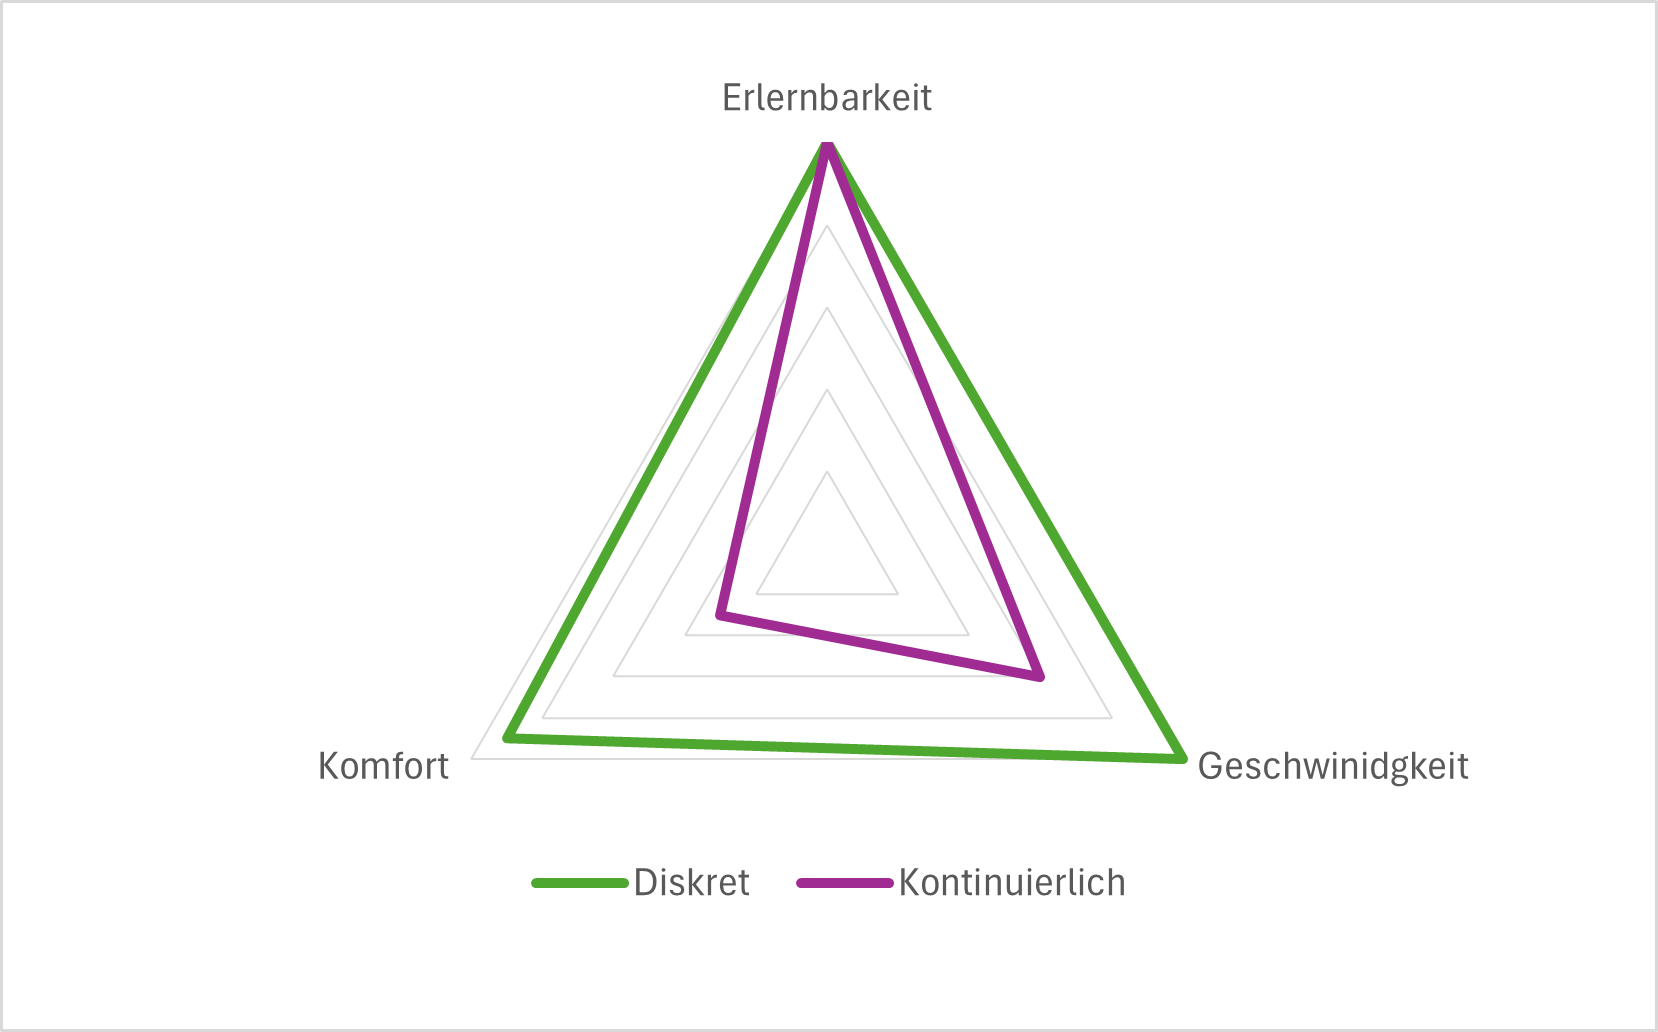
\includegraphics[width=0.75\textwidth]{images/Netzdiagramm-Transition.png}
    \caption{Visualisierung der Einordnung der Gestaltungsoptionen der Interaktionskomponente Transition}
    \label{fig:Netz-Transition}
\end{figure}

\textit{Effizienz:}
Die Effizienz der Interaktion, gemessen am notwendigen Aufwand, wird durch die Gestaltung der Transition kaum beeinflusst. Beide Optionen führen die Rotation mit einem vergleichbaren Aufwand durch, da die grundlegende Interaktion zur Auslösung der Rotation identisch bleibt.

\textit{Effektivität:} 
Die Effektivität der Interaktion, gemessen an der Präzision des Rotationswinkel, wird durch die Gestaltung der Transition nicht beeinflusst. Der exakte Rotationswinkel wird durch die Navigation bestimmt, während die Transition lediglich den visuellen Übergang zwischen Ausgangs- und Zielposition gestaltet.

\textit{Erlernbarkeit:}
Die Erlernbarkeit der Optionen ist als hoch einzuschätzen, da beide Ansätze bereits in etablierten VR-Anwendungen implementiert werden und somit den Nutzenden einen Wiedererkennungswert bieten.
%BEISPIELE EINBINDEN! 

\textit{Robustheit:}
Die Optionen zur Gestaltung der Transition haben keinen bedeutenden Einfluss auf das Auftreten oder die Vermeidung von Fehlern und somit keinen direkten Einfluss auf die Robustheit. Es kann davon ausgegangen werden, dass beide Optionen stabile und zuverlässige Transitionen darstellen, da sie bereits häufig in VR-Anwendungen implementiert sind. Einflüsse auf die Robustheit können sich ggf. ergeben, wenn durch die Art der Transition Motion Sickness auftritt und die Nutzenden in Folge dessen dazu neigen, eher Fehler zu machen. 

\textit{Interaktionsgeschwindigkeit:}
Die Optionen für die Transition unterscheiden sich in der Interaktionsgeschwindigkeit. Direkte Rotation bietet eine schnellere Interaktionsgeschwindigkeit, da die Kamera ohne Übergangszeit unmittelbar in die gewünschte Position gebracht wird. Die kontinuierliche Rotation hingegen ist aufgrund der Übergangszeit langsamer. Hier findet eine Bewegung der Kamera über die Zeit statt. Daher benötigt diese Transition länger, um die Zielposition zu erreichen \citep{8797722}. Der Unterschied zwischen den Interaktionszeiten wird durch die Geschwindigkeit der Kamerabewegung und die Größe des gewählten Rotationswinkels beeinflusst. Eine Rotation um einen großen Rotationswinkel erfordert mehr Zeit. Bei einer Direkten Rotation ist die Geschwindigkeit hingegen konstant und nicht von anderen Faktoren abhängig. 

\textit{Komfort:}
Die Optionen für die Transition unterscheiden sich deutlich in Bezug auf den Komfort, insbesondere im Hinblick auf die Auswirkungen auf die Wahrscheinlichkeit für das Auftreten von Motion Sickness und die räumliche Wahrnehmung.
Die kontinuierliche Rotation ahmt die natürliche Bewegung des Kopfes nach und wird daher als realistischer empfunden \citep{8797722}. Dies kann das räumliche Bewusstsein der Nutzenden verbessern \citep{10.1145/3441852.3471230}. Allerdings birgt die Kontinuierliche Transition ein sehr hohes Risiko für das Auftreten von Motion Sickness \citep{10.1007/s10055-020-00425-x, 8797722}, was den Komfort deutlich mindert.
Im Gegensatz dazu ist das Risiko von Motion Sickness bei der direkten Rotation vergleichsweise gering. Allerdings kann die plötzliche Änderung des Sichtfeldes dazu führen, dass die Nutzenden kurzzeitig die räumliche Orientierung verlieren und sich in ihrer Umgebung neu orientieren müssen \citep{10.1145/3441852.3471230}. 

\textbf{3. Initialisierung} 

Im Folgenden werden die erarbeiteten Gestaltungsoptionen für die Komponente Initialisierung anhand der definierten Parameter eingeordnet. Die Ergebnisse dieser Einordnung sind in \autoref{fig:Netz-Initialisierung}zusammenfassend dargestellt. 

\begin{figure}[tbh]
    \centering
    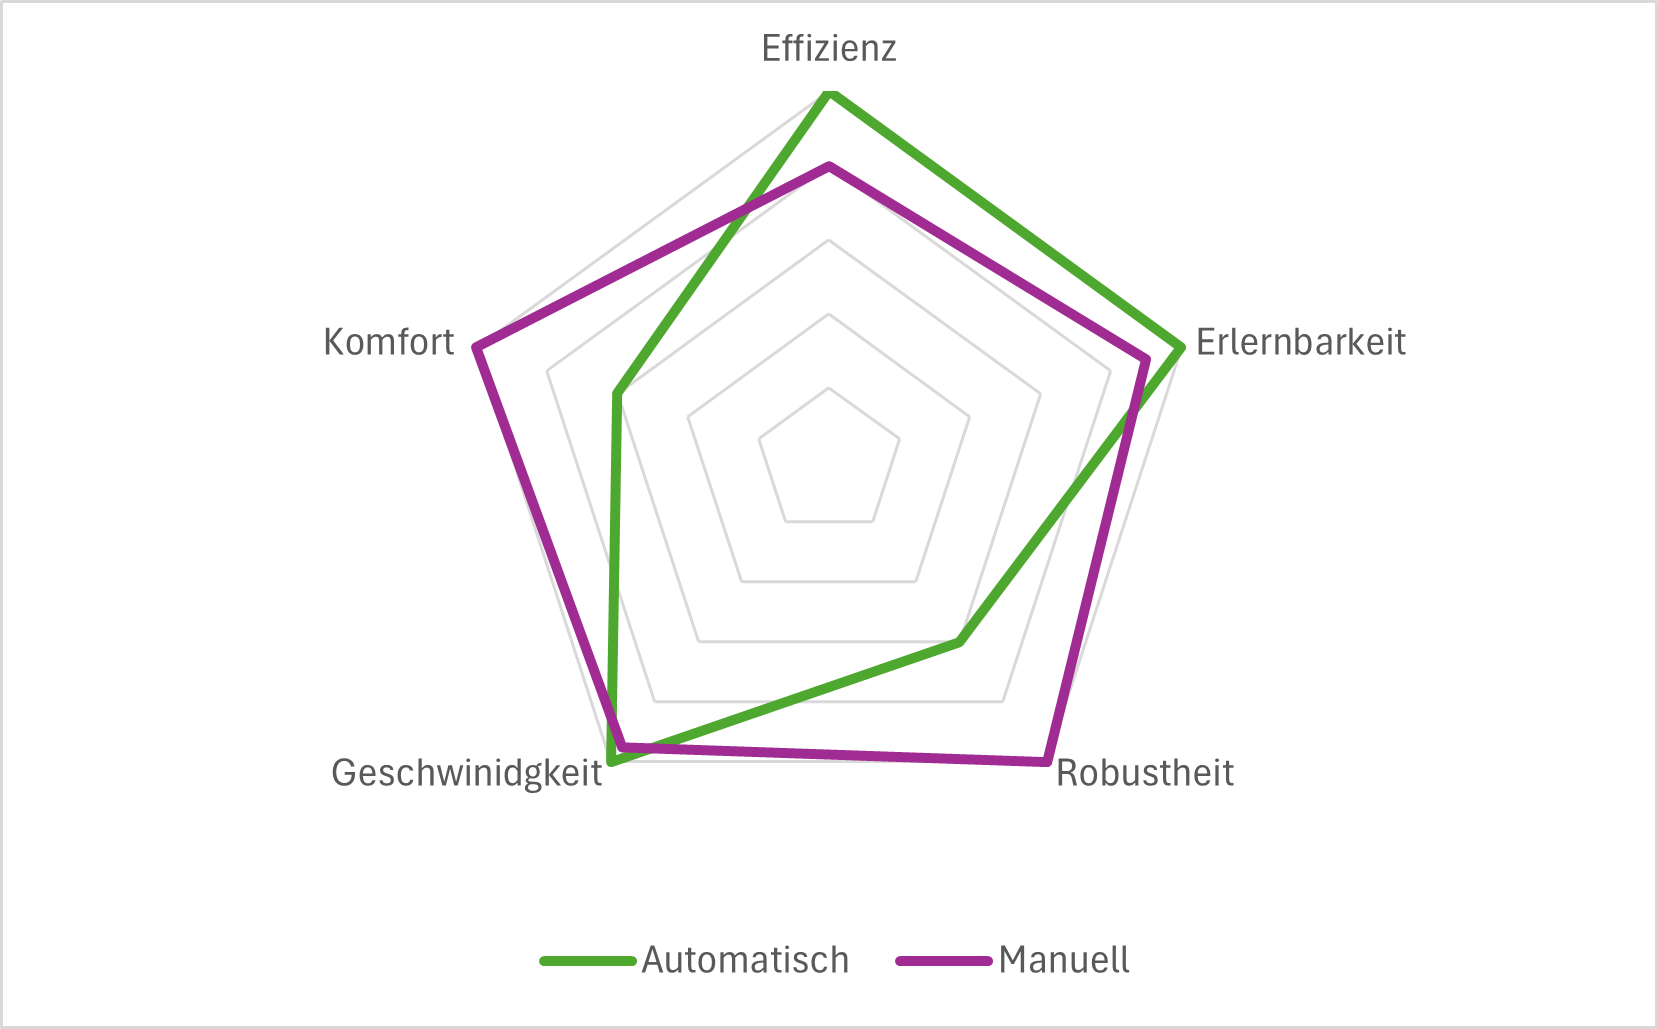
\includegraphics[width=0.75\textwidth]{images/Netzdiagramm-Initialisierung.png}
    \caption{Visualisierung der Einordnung der Gestaltungsoptionen der Interaktionskomponente Initialisierung}
    \label{fig:Netz-Initialisierung}
\end{figure}

\textit{Effizienz:}
Die Effizienz der beiden Initialisierungsoptionen unterscheidet sich nur geringfügig. Die automatische Aktivierung ermöglicht eine kontinuierliche Verfügbarkeit des Scanning-Verfahrens, sodass Interaktionen jederzeit ohne vorherige Aktivierung durchgeführt werden können. Dies reduziert den Aufwand und erhöht die sofortige Bereitschaft für Interaktionen. Die manuelle Initialisierung erfordert hingegen einen zusätzlichen Zwischenschritt, bei dem die Nutzenden das Scanning-Verfahren aktivieren. Obwohl dieser Schritt allein nur minimalen Aufwand erfordert, kann er in Szenarien, in denen häufige Aktivierungen erforderlich sind, den erforderlichen Gesamtaufwand erhöhen. 

\textit{Effektivität:}
Die Effektivität wird durch die Wahl der Initialisierungsoption kaum beeinflusst. Der Initialisierungsschritt bei der manuellen Aktivierung hat keinen Einfluss auf die Genauigkeit oder den Erfolg der Interaktion selbst, sondern nur auf den Beginn des Prozesses.

\textit{Erlernbarkeit:}
Die Erlernbarkeit der automatischen Aktivierung ist besonders hoch, da keine zusätzlichen Schritte oder Erklärungen erforderlich sind. Das Scanning-Verfahren wird automatisch gestartet und läuft kontinuierlich ab, was für die Nutzenden direkt ersichtlich ist. Im Gegensatz dazu erfordert die manuelle Initialisierung eine kurze Einführung, um den Aktivierungsmechanismus zu erklären. Da dies im Allgemeinen durch eine einfache Eingabe erfolgt, bleibt die zusätzliche kognitive Belastung gering und die Erlernbarkeit wird nur minimal beeinflusst.

\textit{Robustheit:}
Die Robustheit der manuellen Initialisierung wird als höher eingestuft, da das Scanning-Verfahren erst nach einer bewussten Aktivierung durch den Nutzenden startet. Dies minimiert das Risiko unbeabsichtigter Eingaben oder Fehlselektionen, die bei einer kontinuierlichen Aktivierung häufiger auftreten könnten. Die automatische Aktivierung hingegen erhöht die Wahrscheinlichkeit von Fehlselektionen, da das Scanning dauerhaft aktiv ist und unbeabsichtigte oder doppelte Eingaben potenziell direkt eine Interaktion auslösen.

\textit{Interaktionsgeschwindigkeit:}
Die Interaktionsgeschwindigkeit wird bei einem durchgehend aktivierten Scanning-Verfahren leicht positiv beeinflusst, da keine zusätzliche Initialisierung erforderlich ist. Die Nutzenden können direkt mit der Interaktion beginnen, was eine schnelle Ausführung ermöglicht. Im Vergleich dazu führt die manuelle Initialisierung zu einem minimalen Zeitverlust durch den zusätzlichen Zwischenschritt, der in der praktischen Anwendung jedoch vermutlich unerheblich ist.

\textit{Komfort:}
Der Komfort ist je nach Initialisierungsoption des Scanning-Verfahrens unterschiedlich. Eine automatische Aktivierung führt zu einer permanenten Überlagerung der Szene mit dem Scanning-Verfahren, was von den Nutzenden als störend empfunden werden könnte. Dies erhöht die visuelle Komplexität und erfordert eine stärkere Konzentration auf den eigentlichen Inhalt der Szene. Darüber hinaus könnte die kontinuierliche Bewegung des Scanning-Verfahrens bei längerer Nutzung ermüdend wirken und die immersive Wahrnehmung der Szene beeinträchtigen.
Im Gegensatz dazu bietet die manuelle Initialisierung den Nutzenden die Möglichkeit, das Scanning-Verfahren nur bei Bedarf zu aktivieren. Dadurch wird die visuelle Komplexität der Szene reduziert, was zu einer entspannteren Nutzung und einer besseren Fokussierung auf wesentliche Inhalte beitragen könnte. Insbesondere bei längerer Nutzung oder bei Szenen mit komplexen visuellen Informationen kann dadurch der Komfort gesteigert werden. Darüber hinaus könnte die zeitweise Deaktivierung des Scanning-Verfahrens ein tieferes Eintauchen in die virtuelle Szene ermöglichen, da weniger Ablenkung durch visuelle Elemente besteht.

\section{Ableitung der finalen Konzepte}
% Wie wurde die Auswahl getroffen (Kriterien), welche Konzepte mit welchen Ausprägungen ergeben sich daraus, welche Strategien werden angewandt, um Problemen entgegenzuwirken (z.b. Item Animation um Scan-Reihenfolge zu visualisieren und damit mehr Orientierung zu liefern, beschränkung Scanning auf Ebenen (Im Menü wird nur Menü durchlaufen, im Dialog nur Antwortmöglichkeiten etc), zurück-option bei Menü; bei Cartesain: wechsel des Modus durch gedrückt halten, verschiedene farben der Scan-Linien um den Modus zu visualiseren, Linien leer durchlaufen lassen bricht den Scan ab, nach einem durchlauf gehts wieder von vorne los)

Die Festlegung der zwei finalen Konzepte für die zwei zu entwickelnden Interaktionsschnittstellen erfolgt auf Basis der detaillierten Bewertung der Gestaltungsoptionen, wie sie im vorangegangenen Abschnitt erarbeitet wurden. Dabei wird diejenige Option bevorzugt, die in der Gesamtbetrachtung die positivsten Bewertungen aufweist und ein ausgewogenes Verhältnis zwischen Effektivität, Effizienz, Robustheit, Interaktionsgeschwindigkeit, Erlernbarkeit und Komfort bietet.
Der Komfort steht dabei besonders im Vordergrund, da das Auftreten von Motion Sickness einen erheblichen Einfluss auf die generelle Nutzbarkeit und Akzeptanz der Interaktionsschnittstellen hat. In den Bereichen, in denen keine der Optionen hinsichtlich der Parameter eindeutig überlegen ist, wird dieser Aspekt entsprechend stärker gewichtet. Damit soll sichergestellt werden, dass die ausgewählten Konzepte nicht nur funktional, sondern auch für die Nutzenden angenehm und zugänglich sind.


{\normalfont \bfseries 1. Konzept: (Automatic) Item Scanning} 

\begin{figure}[tbh]
    \centering
    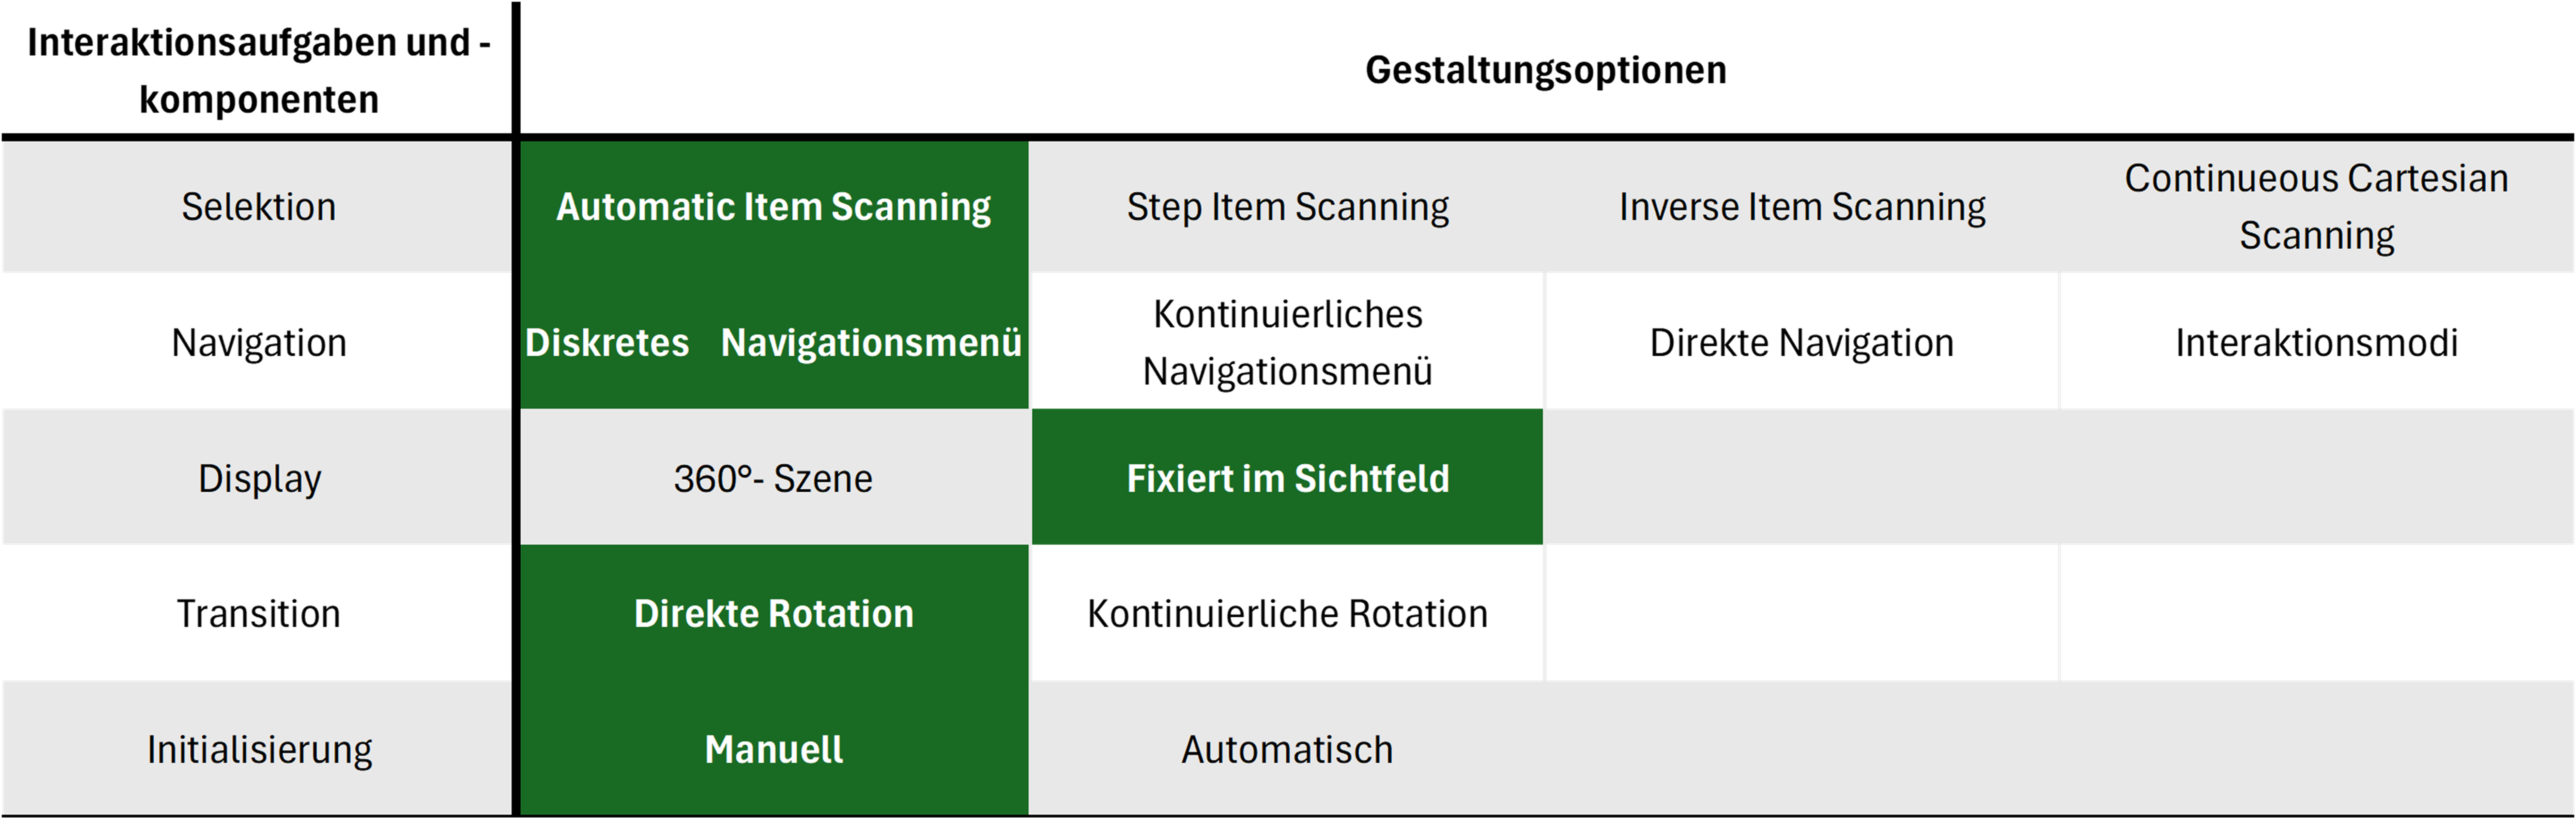
\includegraphics[width=0.95\textwidth]{images/MorphKasten-Item.png}
    \caption{Darstellung des Konzept 1: Item Scanning}
    \label{fig:MorphKasten-Item}
\end{figure}

Das erste Konzept basiert auf dem Automatic Item Scanning , das sich durch eine vergleichsweise ausgewogene Bewertung in allen Parametern auszeichnet. Es erzielt zwar nicht in allen Kriterien die besten Ergebnisse, weist aber insgesamt die geringsten Defizite auf und bietet eine solide Grundlage für eine effektive und effiziente Interaktion. Die Navigation erfolgt über ein diskretes Navigationsmenü. Hier war die Bewertung der Optionen nicht eindeutig, jedoch überzeugt die diskrete Navigation insbesondere durch ihre deutlich geringeren Defizite bezüglich des Komforts. Dies ist insbesondere auf das geringere Risiko von Motion Sickness im Vergleich zur kontinuierlichen Navigation zurückzuführen.

Das Scanning-Verfahren wird im Sichtfeld der Nutzenden fixiert, da diese Gestaltungsoption der Komponente Display hinsichtlich aller Parameter durch klare Vorteile überzeugt. Ebenso wird eine diskrete Rotation als Transitionsmethode verwendet, da diese sowohl hinsichtlich des Komforts als auch der Interaktionsgeschwindigkeit überzeugt. Die Initialisierung des Scanning-Verfahrens erfolgt manuell, da diese Variante im Vergleich zur automatischen Aktivierung zwar eine geringere Effizienz aufweist, aber insbesondere hinsichtlich Komfort und Robustheit Vorteile bietet.
Die für dieses Konzept ausgewählten Gestaltungsoptionen der Interaktionsaufgaben und -komponenten sind in \autoref{fig:MorphKasten-Item} zusammenfassend dargestellt.

Um mögliche Schwächen der gewählten Gestaltungsoptionen zu minimieren, wird das Scanning-Verfahren so gestaltet, dass es nur die Elemente einer aktiven Ebene durchläuft, z. B. nur die Antwortoptionen eines geöffneten Dislog-Elements. Dies reduziert die Größe des Scan-Sets und verkürzt die Interaktionszeit. Zusätzlich wird eine "Zurück"-Option integriert, die es erlaubt, den Dialog durch erneutes Auswählen wieder zu schließen. Um die Orientierung zu verbessern und eine klare Visualisierung der Scan-Reihenfolge zu gewährleisten, wird das Scanning-Verfahren durch eine Animation ergänzt, die die Scan-Reihenfolge verdeutlicht und dadurch die Robustheit erhöht.

{\normalfont \bfseries 2. Konzept: Cartesian Scanning}

\begin{figure}[tbh]
    \centering
    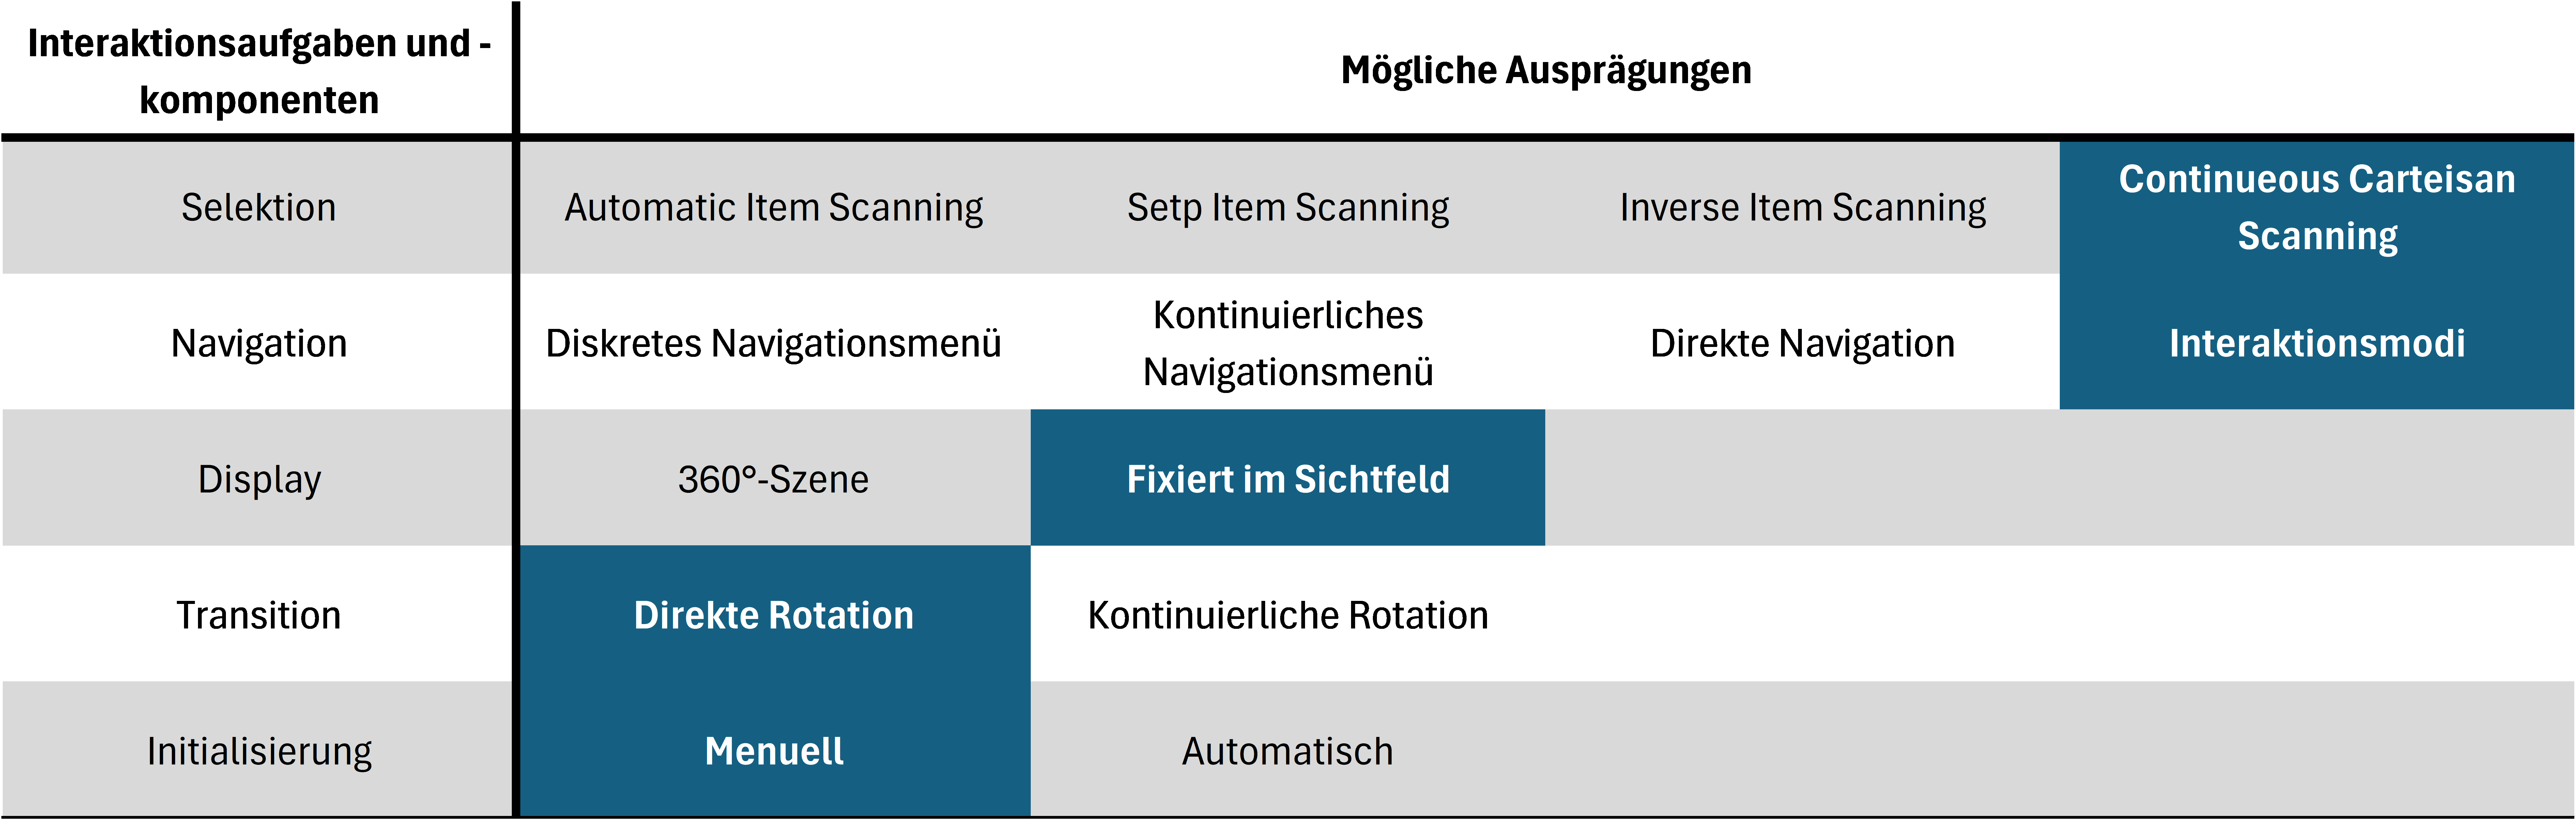
\includegraphics[width=0.95\textwidth]{images/MorphKasten-Cartesian.png}
    \caption{Darstellung des Konzept 2: Cartesian Scanning}
    \label{fig:MorphKasten-Cartesian}
\end{figure}

Das zweite Konzept basiert auf dem Continuous Cartesian Scanning. Die Bewertungen der Selektionsoptionen unterscheiden sich nicht wesentlich. Das Cartesian Scanning wurde bevorzugt vor dem Setp und Inverse Item Scanning ausgewählt, da es insbesondere hinsichtlich Komfort und Effizienz Vorteile aufweist. Für die Navigation werden Interaktionsmodi eingesetzt, da diese Option in den Bewertungen hinsichtlich Robustheit und auch Komfort leicht überlegen ist und eine klar strukturierte Interaktionsführung ermöglicht.
Der Wechsel zwischen den Modi erfolgt durch kurzes Halten des Schalters. Diese Methode hat den Vorteil, dass unbeabsichtigte Wechsel minimiert werden und gleichzeitig eine einfache Bedienung ermöglicht wird. Alternative Wechselmechanismen, wie ein doppeltes Drücken des Schalters oder die Integration eines zusätzlichen UI-Elements in die Szene, wurden verworfen, da sie entweder das Risiko unbeabsichtigter Eingaben erhöhen oder die visuelle Komplexität der Szene unnötig steigern würden.

Auch bei diesem Konzept wird das Scanning-Verfahren im Sichtfeld fixiert und die Transition erfolgt als diskrete Rotation, da diese Gestaltungsoptionen deutliche Vorteile gegenüber den anderen Optionen aufweisen. Die Initialisierung erfolgt auch hier manuell, um unbeabsichtigte Aktivierungen zu vermeiden und den Komfort zu erhöhen.

Die für dieses Konzept ausgewählten Gestaltungsoptionen der Interaktionsaufgaben und -komponenten sind in \autoref{fig:MorphKasten-Cartesian} zusammenfassend dargestellt.

Zur Optimierung des Cartesian Scanning werden unterschiedliche Farben für die Scan-Linien verwendet, um den aktiven Interaktionsmodus klar zu visualisieren. Zusätzlich ist das Scanning-Verfahren so gestaltet, dass die Linien nach ihrem ersten Durchlauf automatisch wieder von vorne beginnen, falls keine Eingabe erfolgt ist. Für den Fall, dass die erste Scan-Linie inkorrekt positioniert wurde, bietet das Verfahren die Möglichkeit, durch bewusstes mehrmaliges Durchlaufen der zweiten Scan-Linie den Scan abzubrechen und die Auswahl zurückzusetzen. Diese Maßnahmen dienen insbesondere der Steigerung der Robustheit.

{\normalfont \bfseries Zusammenfassung}

In diesem Kapitel wurde die Konzeption der Interaktionsmethoden durch eine systematische Analyse und Auswahl von Gestaltungsoptionen entlang definierter Parameter konkretisiert. Dabei wurden zwei Konzepte entwickelt, die auf den jeweiligen Stärken der analysierten Optionen aufbauen und durch gezielte Maßnahmen zur Kompensation möglicher Schwächen ergänzt werden. Während das erste Konzept auf dem Scanning-Verfahren Automatic Item Scanning basiert, wird für das zweite Konzept Continuous Cartesian Scanning als grundlegendes Interaktionsverfahren zur Selektion und Navigation gewählt. Im weiteren Verlauf der Arbeit werden die Konzepte als Vereinfachung über die verwendeten Scanning-Verfahren referenziert. 

Im folgenden \autoref{chap:Implementierung} wird die konkrete Umsetzung dieser Konzepte einschließlich der technischen Umsetzung der gewählten Gestaltungsoptionen sowie der definierten Kompensationsstrategien vorgestellt.